\chapter{IMPLEMENTATION AND DESIGN}
\label{ch:implementation-design}

\sepfootnotecontent{fn:unity-engine}{[Footnote: What is the Unity engine]}

\sepfootnotecontent{fn:triple-a}{AAA (pronounced "triple A") games are an informal classification of video games distributed by major publishers and distinguished by large development and marketing budgets. In general, the term is used to represent the games that are supposed to achieve the highest standard of quality and content in video games.}

\sepfootnotecontent{fn:genshin-impact}{Genshin Impact (miHoYo, 2020). Video Game. Android, iOS, Windows, PlayStation 4, Playstation 5, Nintendo Switch.}

\sepfootnotecontent{fn:escape-tarkov}{Escape from Tarkov (Battlestate Games, 2017). Computer Game. Microsoft Windows.}

\sepfootnotecontent{fn:hollow-knight}{Hollow Knight (Team Cherry, 2017). Video Game. PlayStation 4, Nintendo Switch, Xbox One, macOS, Linux, Microsoft Windows.}

\sepfootnotecontent{fn:ghost-tale}{Ghost of a Tale (SeithCG \& Plug In Digital, 2016). Video Game. PlayStation 4, Nintendo Switch, Microsoft Windows, Xbox One.}

\sepfootnotecontent{fn:cuphead}{Cuphead (Studio MDHR Entertainment Inc., 2017). Video Game. PlayStation 4, Nintendo Switch, Xbox One, Microsoft Windows, macOS.}

\sepfootnotecontent{fn:undead}{\emph{Undead} beings are fictional characters represented by entities that were reanimated from death through supernatural means. Common representations of \emph{Undead} beings in popular media include \emph{Zombies}, \emph{Skeletons} and \emph{Vampires}.}

\sepfootnotecontent{fn:particle-vfx}{Footnote: What are particle-based visual effects}

\sepfootnotecontent{fn:death-stranding}{Footnote: What is Death Stranding}

\sepfootnotecontent{fn:core-gameplay-loop}{Footnote: What is the Core Gameplay Loop}

\sepfootnotecontent{fn:character-controller}{Footnote: What are CharacterControllers}

\sepfootnotecontent{fn:movement-drifting}{Footnote: What is movement drifting}

\sepfootnotecontent{fn:lock-on}{Footnote: What is Lock-On targeting}

\sepfootnotecontent{fn:colliders}{Footnote: What is a collider}

\sepfootnotecontent{fn:collider-overlapping}{Footnote: What is collider overlapping}

\sepfootnotecontent{fn:monobehaviour}{Footnote: What is a MonoBehaviour}

\sepfootnotecontent{fn:fixed-update}{Footnote: What is the FixedUpdate timestep}

\sepfootnotecontent{fn:rays}{Footnote: What are rays}

\sepfootnotecontent{fn:raycasts}{Footnote: What are Raycasts}

\sepfootnotecontent{fn:mecanim}{Footnote: What is the Mecanim system}

\sepfootnotecontent{fn:skeletal-rigs}{Footnote: What are skeletal rigs}

\sepfootnotecontent{fn:motion-sickness}{Footnote: What is motion sickness}

\sepfootnotecontent{fn:unity-prefabs}{Footnote: What are Unity Prefabs}

\sepfootnotecontent{fn:unity-gameobjects}{Footnote: What are Unity GameObjects}

\sepfootnotecontent{fn:transposing-and-composing}{Footnote: What are Transposing and Composing strategies}

\sepfootnotecontent{fn:observer-pattern}{Footnote: What is the Observer pattern}


% * ===================================================================
% * ===================================================================
% * ===================================================================

% About our implementation of Dark Souls "Core"
In this chapter, we specify each of the major decisions taken to implement a minimalistic "Souls-like" game based on the original Dark Souls, with an additional adaptive system that dynamically adjusts game difficulty to the profile of players. We provide a detailed list of the requirements of our implementation, along with the motivation for the choice of each technology.

% Criteria for third-party assets
% Limitations to original game
We formulate our criteria for the use of third-party dependencies, including visual and audio assets which greatly improved the development speed of our application. We also specify the technical design and implementation of all major gameplay systems in our implementation, and explain the inherent limitations of the scope of this work, along with the consequential differences to the original game. 

% About our implementation of DDA
We detail our implementation for an event tracking system which monitors actions performed by in-game entities, and address how it is used as infrastructure for our DDA system. We specify the in-game events which are captured by the event tracking system, and how such events are converted to metrics that serve as input for our adjustment policies. We elicit the in-game modifications that each adjustment performs, and how such modifications can affect a gameplay session.

% * ===================================================================
% * ===================================================================
% * ===================================================================

\section{Tools and Frameworks}

% Brief overview of tools used in the project, specify that we chose Unity, Cinemachine, Post Processing Stack, Aura Volumetric Rendering

\sepfootnotecontent{fn:unity-engine}{\emph{Unity} is a cross-platform game engine which provides reusable functionality for rendering, input handling, audio and gameplay systems. Unity is widely used in the games industry due to its simplicity for beginner developers, being a popular choice for independent game development.}

To implement a subset of Dark Souls that satisfies our purposes of evaluating DDA systems, we decided to use a framework able to render 3D environments with high visual fidelity. We also included utilities that would help implement the player interface aspects of the original game, such as an Input System that can deal with multiple input devices, a set functions to manipulate 3D Camera behavior and a physics engine that can detect and handle collisions for at least basic geometry. For these reasons we chose \emph{Unity}\sepfootnote{fn:unity-engine} as our development platform, as it contains most of the essential functionality we require and the possibility of extending and adapting the purpose of its editor to satisfy any development purpose.

% - A concise integrated editor that can be used for map editor, project folder organization, game data management;
Unity offers a concise, integrated project editor that offers functionality such as level editing, game data serialization, visual animation state machines, configuration options for deploying platforms and architectures, a debug console and tools for generating offline light mapping data for scene rendering.

% - A general API that provides the tools to implement virtually any type of game;
% - Possibility to deploy in multiple platforms (Windows, Linux, macOS) with minimal changes in source code;
Unity also defines a streamlined API where developers can implement their custom game code in \textsc{C\#}, providing access to reusable functionality libraries and systems such as the component-based \textsc{MonoBehaviour} API, the \textsc{ScriptableObject} API for serialized game data, the Input and UI systems and even the Editor package, which permits the developer to extend the built-in functionality of the Unity Editor to develop Quality of Life tools for improved creation workflows. It is also possible to deploy Unity projects to multiple platforms such as Windows, Linux, macOS, PlayStation, Nintendo Switch and Xbox with minimal changes in code, as Unity's standardized API and builtin \textsc{IL2CPP} compiler translates Intermediate Language code into native \textsc{C++} tailored for each platform.

% Footnote: Unity Asset Store
\sepfootnotecontent{fn:unity-asset-store}{Unity Asset Store is a digital platform for the distribution and acquisition of game assets such as 3D Models, Animations, Sounds, 2D UI Elements, Shaders, Post-Processing Effects and Visual Effects. Usage of the assets purchased in the platform is restricted to Unity projects, and have individual licensing and usage policies.} 

% - Possibility to import free and paid assets from the Unity Asset Store for 3D Models, Animations, Sounds, UI Elements, Shaders, Post-Processing Effects, Visual Effects;
Another key factor for the choice of Unity was the possibility to import assets from the \emph{Unity Asset Store}\sepfootnote{fn:unity-asset-store}. Without this, it would be impossible for the authors of this work to develop a game that would resemble the qualities of a AAA game such as Dark Souls, or even perform a similar project in a feasible time window. By acquiring and importing high-quality and ready to use game assets into the project, it was possible to focus on the design and development of game systems and our DDA implementation, while also having AAA quality assets as a resource to work with.

% - Authors had previous familiarity with the engine from personal and professional experience;
The final deciding factor for the choice of Unity as a development platform was the previous experience of the authors with the engine, having implemented a wide variety of 2D and 3D Games, VR Serious Games and data visualization tools under the Unity engine. The familiarity with the provided APIs, along with the knowledge of how to achieve a steady and concise workflow permitted the authors to plan a moderately robust architecture and select the appropriate tools to implement the core features of Dark Souls with an acceptable quality.

% ========================================================================
% ========================================================================
% ========================================================================

\section{Game Assets and Aesthetics}

% 3D Models, animations and sound assets were selected based on trying to replicate the same general 'feel' of Dark Souls
The assets used in our implementation were elected to serve as resources as an attempt to replicate the unique aesthetics of Dark Souls. Therefore, as a basis criteria for the selection of used assets, we use the brief analysis in section \ref{sec:analysis-dark-souls} as a reference to explore options in the Unity Asset Store within the \emph{'Dark Fantasy'} thematic subcategory.

% Fantasy Dungeon
First, we require a set of 3D models to assemble a playable 3D environment that satisfies the aesthetics of the 'Dark Fantasy' genre. For this purpose, we chose \emph{Fantasy Dungeon} as our main environment assets source -- a collection of 3D models with a 'Ruined Castle' theme. The aesthetical aspect of this asset pack appropriately resembles the sense of \emph{decay} and \emph{abandonment} in the original game. When considering functionality aspects, this pack contains modular 3D objects and pieces that can be easily assembled into a playable environment. Furthermore, the asset pack also contains pre-assembled scenes with appropriate lighting and optimized meshes, which were adapted to fit the requirements of our implementation.

% Figure: Assets used in setting up the environment
\begin{figure}
    \caption{A selection of screenshots from pre-assembled scenes using the 3D assets from the Fantasy Dungeon asset pack.}
    \begin{center}
        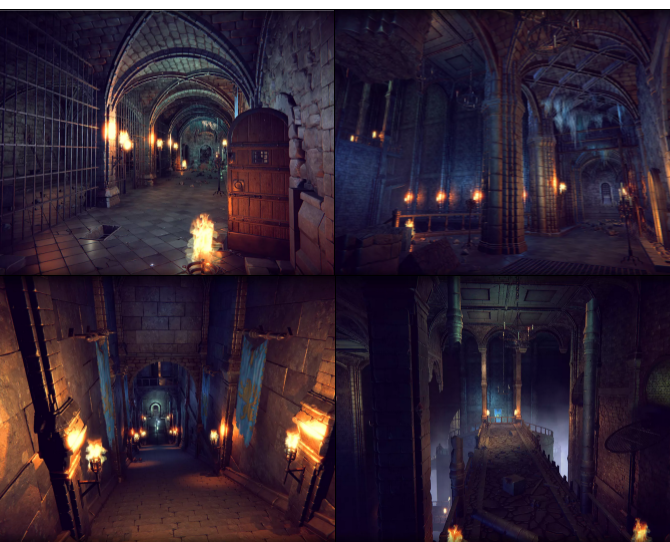
\includegraphics[width=24em]{figures/fig-environment-assets.png}
    \end{center}
    \legend{Source: Collation of screenshots performed by the authors from images captured from the original Unity Asset Store website pages for the \emph{Fantasy Dungeon} Unity asset.}
    \label{fig:environment-assets}
\end{figure}

% Then, we need 3D models for the Characters, The Blacksmith: Characters, Skeleton Zombies and Longsword Animset Pro

In sequence, we require 3D models to represent the player and any non-playable entities the player would be able to interact with. Regarding non-playable entities, we attempt to implement enemy agents comparable to the enemies presented in the early levels of Dark Souls. Most of the enemies in these early sections of the original game are \emph{Undead}\sepfootnote{fn:undead} beings named \emph{'The Hollow'}, which are represented by creatures with decomposed skin and a dehydrated body that resemble \emph{Zombies}. In the original game, \emph{The Hollow} can be seen wearing a variety of attire, including ragged clothes, armored pieces such as cuirasses, pauldrons and helmets, bare skin or even without flesh in their bodies in the form of \emph{Skeletons}.

In addition to the requirement of being in harmony with the aesthetics of the original game, we also used as selection criteria of enemy models their specific purposes in enemy behavior design. Each enemy agent in our game has a specific set of actions which can complement the actions of other enemies during a combat encounter. Therefore, we define enemy role archetypes based on the enemies seen in the initial levels of Dark Souls: the \emph{Ghoul}, the \emph{Archer}, the \emph{Swordsman} and the \emph{Assassin}.

For the representation of enemy characters that satisfy our aesthetic and design requirements, we selected \emph{Skeleton Zombies}, \emph{Longsword Animset Pro}, \emph{Modular Skeleton Archer}, \emph{Modular Skeleton Rogue} and \emph{Skeleton Humanoid} as our enemy assets, all of which contain 3D models representing stereotypes of Zombies and Skeletons that resemble the enemies seen in the early stages of Dark Souls, while satisfying the roles we defined for the design of enemy agents in our implementation.

Another motivation for the selection of these assets was their compatibility with the \textsc{Mecanim}\sepfootnote{fn:mecanim} system, which standardizes \emph{skeletal rig}\sepfootnote{fn:skeletal-rigs} definitions for animations in humanoid characters in the \textsc{Unity} engine. When compatible with this system, character models can be used in combination with most animations that can be found in the \textsc{Unity Asset Store}, which provides the possibility of choosing from a wide collection of animation sets, which also assists our enemy behavior design.

% Figure: Assets used for character models
\begin{figure}
    \begin{center}
    \caption{A mosaic portraying the 3D character models in Bright Souls.}
        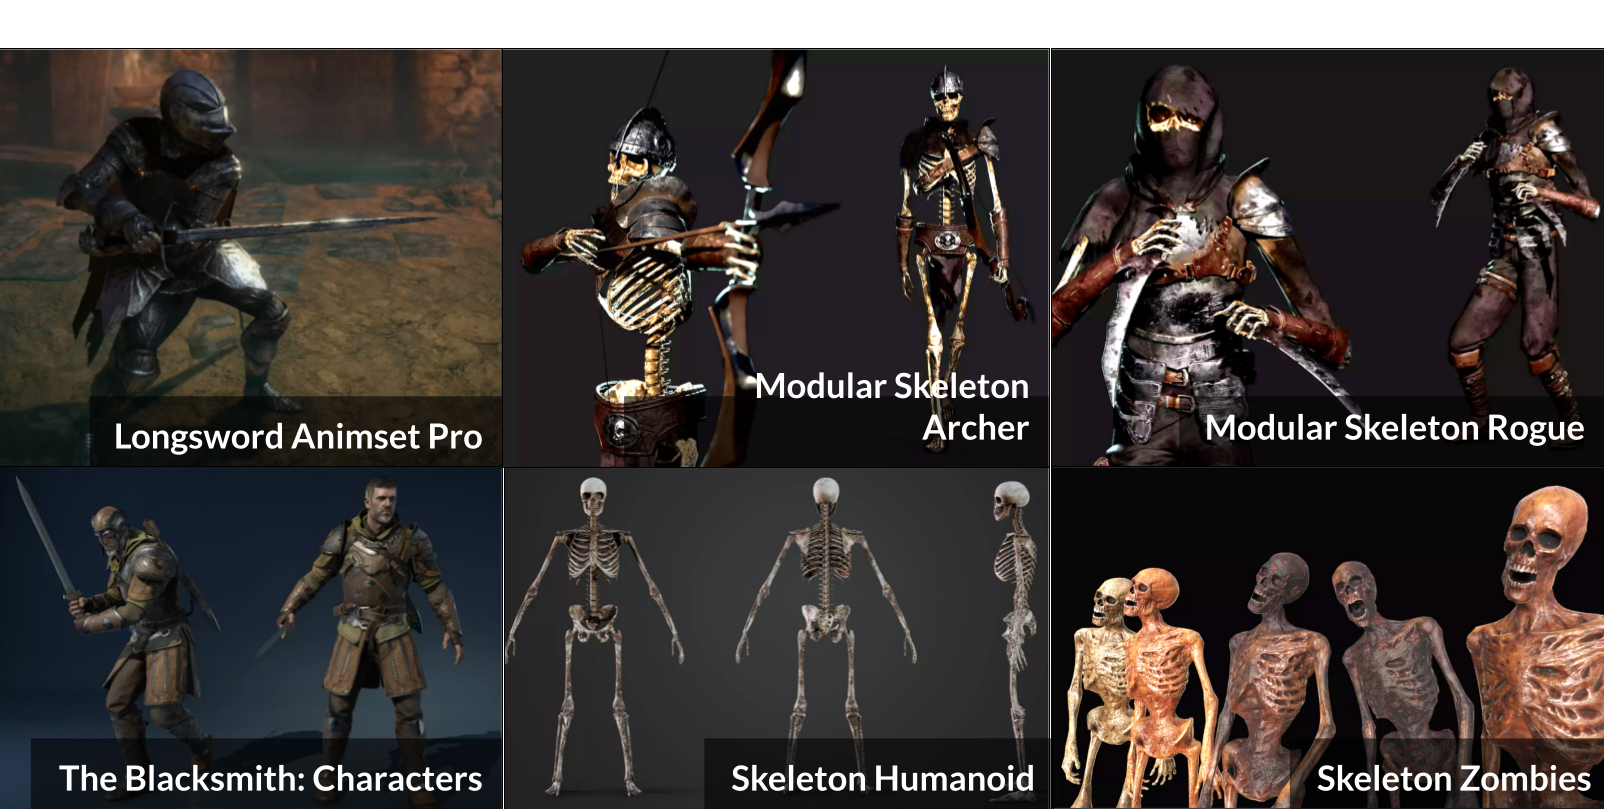
\includegraphics[width=30em]{figures/fig-character-assets.png}
        \legend{Source: Collation of screenshots performed by the authors from images captured from the original Unity Asset Store website pages for each of the assets used in this work.}
    \end{center}
    \label{fig:character-assets}
\end{figure}

% Talk about model for player Character: Blacksmith: Characters
When considering the options for the player model, we require a character that would equip the appropriate attire or armor pieces, and should be able to wield common Fantasy-genre weapons such as swords and shields. The second criteria considers the gameplay aspects of our implementation, where we require animations that represent a subset of combat and movement animations from the original game. In our case, we restricted combat equipment to using the most popular player setup -- the "Sword \& Shield" combination.

We filtered our search to a 3D model for a humanoid character that satisfies the \emph{Warrior} character archetype wielding a sword and shield, and that was compatible with the skeletal rig for an animation set that contains sword and shield animations. For this purpose, we selected the \emph{Challenger} character model from the \emph{Blacksmith: Characters} asset pack, which portrays a middle-aged warrior wielding a sword and shield and using leather body armor pieces. As with the 3D models selected for non-playable entities, the Challenger character is compatible with the \textsc{Mecanim} skeletal rig system from Unity, which provided compatibility with most animation asset packs from the \textsc{Unity Asset Store}.

% After that, we need animations that can be easily integrated with the designed combat system
To properly integrate the characters into the game world, and to provide visual feedback as to what actions characters are performing, we required animations for humanoid characters to be compatible with the \textsc{Mecanim} system and congruent with the purpose of each target entity. The animation set for each playable or non-playable character should appropriately reflect the equipment that each character possesses, the character's body proportions and the weight of the attire being used.

An example of animations being congruent with the purpose of a character would be an archer enemy that has animations for wielding a bow, drawing arrows from a quiver and shooting arrows. Since the armor pieces for an archer enemy should be lighter in comparison to a heavy-armored warrior archetype enemy, the movement animations should include faster steps and less restricted joint rotations to reflect the weight of the light attire.

Considering these requirements, we selected the asset packs \emph{ZOMBIE Starter Animation Set}, \emph{Sword and Shield Animset Pro}, \emph{Longsword Animset Pro}, \emph{Archer Animset Pro} and \emph{Rogue Animset Pro}. Each of the animation sets selected satisfied the functional requirements of a specific role for both playable and non-playable characters, while also being compatible with the skeletal rig standard defined by the \textsc{Mecanim} system.

% Then, we need sound effects and ambient background music that mirror the affective purpose of sound in Dark Souls
We also required sound effects to provide a clear feedback of actions and consequences in the game world, such as a character moving, attacking, blocking an attack, getting hit by an attack or dying. The sound effects for our implementation were selected mainly because of their similarity to the sound effects of the equivalent effects in the original game. For instance, a sound effect for when a character is hit in the original game conveys both the weapon that is being used by the attacker and the scale of damage that is being applied to the target. A frontal attack presents less of a deep, impactful sound effect than a back-stab attack, which does a significantly higher amount of damage. For these reasons, we chose the asset packs \emph{Axe Swing \& Damage Sounds}, \emph{Medieval Fantasy 2 Audio} and \emph{Universal Sound FX} which contain a wide variety of sound effects representing medieval melee weapons such as swords, axes, shields and bows, while also providing a variety of impact levels for successful attacks.

The immersion of players was also considered, and thus we chose to add ambient background noises and music that could be looped for the duration of a session. For the selection of these noises, it was decided that they should provide a sense of depth to the scenery, with quieter sound effects for events that are closer to the player such as crumbling stone and crackling wood, and somewhat louder sound effects for events that are far away from the player, such as running water, fire and falling chunks of stone. As for the music, it should provide an overall sense of horror and mystery that goes in accordance with exploration in a Dark Fantasy world. Therefore, we selected the asset packs \emph{Medieval Fantasy 2 Audio} and \emph{Dark Fantasy Audio} for ambient sound effects and music, which can appropriately convey the sense of an abandoned, crumbling castle while also containing music for an eerie environment.

% We also need Visual Effects that can go along with the sound effects to provide a proper visual feedback when the player hits an enemy. % 

In sequence, we required a collection of \emph{particle-based}\sepfootnote{fn:particle-vfx} visual effects to provide a proper visual feedback when characters are able to successfully attack their enemies, as well as visual effects that complement the aesthetics of the 3D environment. For conveying successful attacks, we chose to add pseudo-volumetric particles for splatters of blood that originate from the body of an attacked entity, with the asset pack \emph{Pseudo-Volume Blood Effects} being the most appropriate for this purpose. To increase the detail and depth of our 3D environment, we used fire particle effects for candle and small torches from \emph{Smoke \& Ember FX} and \emph{Unity Particle Pack}. In additional to fire particles, these asset packs also provided smoke particle effects, which were used to both complement the fire from light sources and to help occlude certain parts of our levels until the player moved to a closer position.

% We need 2D UI Elements that can convey the basic gameplay resources: Health and Stamina
We also needed a collection of 2D UI Elements that would be able to convey the basic player resources such as \emph{Health} and \emph{Stamina}. The standardized solution of \emph{Health Bars} suffices for both attributes, as they are commonly used for representing attributes that have a variable maximum value and a minimum value of zero. We required the design and layout of these elements to resemble the original game, avoiding overly saturated color pallettes and exaggerated visual complexity.

% We also need UI Elements for menus, settings, tooltips and button captions
We also required a variety of UI elements to assemble the menus that will be used by the player to initiate sessions, pages for the configuration of game settings, small tooltips that provide a brief description of the functionality of UI elements, and button captions that can be displayed during a game session to provide the player with a reference of the actions that can be performed at any given time.

To represent most of the UI elements in our implementation we selected the  \emph{RPG \& MMO UI 5} asset pack, which contains the most common UI elements used in the video games such as menus, buttons, tooltips, health bars, loading screens and portraits, and has an overall design tailored for Fantasy-themed games. This asset pack also contains an under-saturated color palette with greyed out colors, which goes in accordance with our Dark Fantasy aesthetic. For button captions we selected the \emph{PC \& Consoles Buttons Icons} asset pack, which contains button icons for a multitude of input devices such as Xbox Controllers, PlayStation Controllers, Mouse \& Keyboard and even joysticks for Head-Mounted devices.

% Finally, we used complementary editor tools that allowed for a more concise and streamlined workflow for serializing game data and implementing common functionality for third-person hack and slash games
We also included \emph{Odin Inspector} as a complementary asset editor tool that allowed for a more concise workflow when serializing game data such as character attributes, physics properties and gameplay values into binary game asset files. With \emph{Odin Inspector}, it was possible to create reusable serializable interfaces that could be assigned to components directly from the \textsc{Unity} engine editor, which was used as a base for the creation of our \emph{Attributes}, \emph{State Machines} and \emph{Performance Tracking} systems.

% Table showing Asset Name, Type, Size, Price, Path in Project
In conclusion, we specify our chosen assets, plugins and frameworks in table \ref{tab:table-game-assets} to provide a consolidated list of the elements discussed in this section, along with the appropriate extraction paths for the assets to work with our source code.

% Table: List of game assets
\begin{table}[!h]
    \begin{center}
      \caption{A consolidated list of the assets used in the implementation of this work.}
      \label{tab:table-game-assets}
      \rowcolors{2}{}{gray!25} % Alternate row colors
      \begin{tabular}{ >{\small}w{l}{11em} >{\small}w{c}{4em} >{\small}w{c}{3em} m{13em} } % alignments and column size
        \addlinespace
        \toprule
        % Headings
        \textbf{Name}                & \bf Type  & \bf MSRP & \textbf{\small Path in Project}                             \\
        \midrule
        % 3D Models
        Fantasy Dungeon              & 3D Models &  \$90.00 & \texttt{\tiny Assets/AssetStore/3D/FantasyDungeon/}      \\ 
        Skeleton Zombies             & 3D Models &  \$16.00 & \texttt{\tiny Assets/AssetStore/3D/StudioNewPunch/}      \\
        Modular Skeleton Archer      & 3D Models &  \$34.99 & \texttt{\tiny Assets/AssetStore/3D/SkeletonArcher/}      \\
        Modular Skeleton Rogue       & 3D Models &  \$34.99 & \texttt{\tiny Assets/AssetStore/3D/SkeletonRogue/}       \\
        Skeleton Humanoid            & 3D Models &  \$19.99 & \texttt{\tiny Assets/AssetStore/3D/SkeletonHumanoid/}    \\
        The Blacksmith: Characters   & 3D Models &     FREE & \texttt{\tiny Assets/AssetStore/3D/ChallengerCharacter/} \\
        \midrule
        % Animations
        ZOMBIE Starter Animation     & Animation &   \$4.99 & \texttt{\tiny Assets/AssetStore/3D/ZombieAnimset/}       \\
        Sword and Shield Animset Pro & Animation &  \$65.00 & \texttt{\tiny Assets/AssetStore/3D/SwordShieldAnimset/}  \\
        Longsword Animset Pro        & Animation &  \$50.00 & \texttt{\tiny Assets/AssetStore/3D/LongswordAnimset/}    \\
        Archer Animset Pro           & Animation &  \$55.00 & \texttt{\tiny Assets/AssetStore/3D/ArcherAnimset/}       \\
        Rogue Animset Pro            & Animation &  \$50.00 & \texttt{\tiny Assets/AssetStore/3D/RogueAnimset/}        \\
        \midrule
        % Sound effects and Music
        Axe Swing \& Damage Sounds   & SFX       &   \$5.00 & \texttt{\tiny Assets/AssetStore/Audio/AxeSwingSounds/}   \\
        Medieval Fantasy 2 Audio     & SFX       &  \$50.00 & \texttt{\tiny Assets/AssetStore/Audio/MedievalFantasy2/} \\ 
        Universal Sound FX           & SFX       &  \$40.00 & \texttt{\tiny Assets/AssetStore/Audio/UniversalSoundFX/} \\
        \midrule
        % Music
        Dark Fantasy Audio           & Music     &  \$22.99 & \texttt{\tiny Assets/AssetStore/Audio/DarkFantasyAudio/} \\
        \midrule
        % Visual Effects
        Pseudo-Volume Blood Effects  & VFX       &  \$15.00 & \texttt{\tiny Assets/AssetStore/VFX/KriptoFX/BloodFX/}   \\ 
        Smoke \& Ember FX            & VFX       &  \$10.00 & \texttt{\tiny Assets/AssetStore/VFX/SmokeEmberFX/}       \\ 
        Unity Particle Pack          & VFX       &     FREE & \texttt{\tiny Assets/AssetStore/VFX/UnityParticlePack/}  \\
        \midrule
        % UI Elements
        PC \& Consoles Buttons Icons & UI        &  \$14.99 & \texttt{\tiny Assets/AssetStore/UI/PCConsolesIcons/}     \\ 
        RPG \& MMO UI 5              & UI        &  \$35.00 & \texttt{\tiny Assets/AssetStore/UI/RPGMMOUI5/}           \\
        \midrule
        % Editor Utilities and Extensions
        Odin Inspector               & Plugin    &  \$55.00 & \texttt{\tiny Assets/Plugins/Sirenix/}                   \\ 
        \bottomrule
      \end{tabular}
    \end{center}
  \end{table}

% ========================================================================
% ========================================================================
% ========================================================================

\section{Gameplay Mechanics and Systems}

% Overview of all gameplay subsystems
% - Here we talk about the subsystems that involve the player-controlled character in our implementation and how it interacts with non-playable entities
In this section, we detail our implementation regarding the subsystems that involve player input and its resulting actions on the player-controlled character and camera. We also specify how such actions might interact with the environment, interactable objects and AI agents in our simulation.

% - Movement mechanics with collision handling for walls and obstacles, detection of slope thresholds and handling of gravity and fall damage
% - A character animation systems that reacts to actions performed by the player and any events that might affect the status of the player, such as hits taken, staggering and death
% - A third person camera that allows the player to orbit the viewport around the game character, while also constraining its position and viewport contents to the boundaries of a playable environment
% - A lock-on camera that is able to frame the player and a target enemy character, and which is coupled with a target prioritization system for enemy characters, and that allows the player to switch targets
% - A combat system which handles hit and block detection, combat effects such as stamina draining, damage and poise break, attack action and state handling, and combat statuses that affect the ability of a character performing actions
% - An attributes system that can be containerized into components for game entities, is able to serialize value data types, broadcasts events when its values are changed, and can be used by other gameplay subsystems to determine the status of a game entity
% - A character status system that accounts for Invincibility Frames (IFrames) when dodging and the inability of performing actions when staggered or dead

% ========================================================================
% ========================================================================
% ========================================================================


\subsection{Camera System}
\label{sec:lock-on-camera}

% In this implementation, we design and implement two separate camera modes
%   - Orbital Third Person Camera
%       > Commonly used for third person hack n' slash or platforming games
In our implementation, we use our analysis of \emph{Dark Souls} in section \ref{sec:analysis-dark-souls} to design two separate camera modes with complementary functionality be used by the player for exploration and combat. First we implement an \emph{Orbital Camera}, which is commonly used in third person \emph{Hack and Slash} and \emph{Platforming} games. Orbital Cameras can be used by the player to evaluate the properties of the environment, quickly assess dangers and devise a plan of action.

%       > In our game, it is the default camera mode, used for traversal around the map
%       > Free control over framing enables player to scout for enemies, avoid pitfalls
The Orbital mode is the default camera state in our implementation, and is mainly designed for traversal around the three-dimensional environment. Control over the positioning and framing of the camera which is independent to character movement enables the player to scout the environment for dangerous entities before performing movement. Additionally, the distance from the player character enables the possibility to view enemies behind wall corners, with the player out the sight. Thus, orbital cameras are optimal in out-of-combat situations, as players can gather information safely and devise a plan-of-action.

%       > Camera positions itself in the perimeter of an ellipsoid that is centered on the player
%       > Input from the player generates movement along the perimeter, causing the camera to orbit around the player
%       > Attempts to frame both the player and the environment by using a position above the player as pivot
An Orbital Third Person Camera is always positioned in the perimeter of a three dimensional ellipsoid centered on the player. Input from the player generates movement along such perimeter. The camera attempts to frame both the player and the environment at the same time, targeting a pivot slightly above the player character's head as a rotation center. Rotations around such pivot result in an orbital movement.

%   - Lock-On camera
%       > Mostly used in action third person hack n' slash games that have melee combat, although some RPGs also use it
%       > Camera positions itself behind the player and attempts to frame both the player and a target character
The second camera mode in our implementation is the \emph{Lock-On} state, which is commonly seen in \emph{Hack and Slash} with melee combat. This type of camera positions itself behind the player character, and attempts to frame both the player and a target -- most commonly an enemy character. Whenever the target character moves, the camera adjusts its position and framing to maintain a fixed relative position between the player and their target.

%       > Camera positioning and framing creates fixed "dimensions of movement" of the player relative to a target,
%         making it easier for a player to avoid attacks from that target and find the optimal spacing to land their
%         own attacks
A Lock-On Camera creates fixed axes of movement between the player and their target. If the player's movement input is horizontal, their character moves in a circle around the target. Moving forward and backwards adjusts the distance between the player and their target. The purpose of this mechanism is for the player to have better control of spacing during combat, easing avoidance of attacks and optimization of distance to succesfully strike opponents.

%       > Useful for the player to be able to track and attack a single target with ease without missing,
%         instead of having to specify a "direction" for the attack, the player can simply press the attack button
%         and the character will already be facing the enemy and perform the attack in the correct direction
In the Lock-On Camera State, players do not specify an input direction for attacks. Instead, simply pressing the attack button guarantees a correct attack direction, as the player character constantly faces the enemy. Such simplicity helps the player to focus on enemy actions, to perceive when an enemy is attacking and to identify which kind of attack is being executed.

%       > Has issues in environments in constrained spaces, where the enemy is too close to the player or the player
%         is too close to a wall. Framing becomes an issue in this case
In gaming culture, Lock-On cameras are commonly known for poor framing in specific situations. When the player is too close to their target, camera orientation is often angled towards an unsatisfactory direction. This causes the player to have limited information about their surroundings, hindering the ability to efficiently dodge enemy attacks, or even to navigate the environment. Furthermore, if a player is moving horizontally when overtly close to their target, the perimeter of the circle of movement has a reduced radius in comparison to higher distances. This causes the camera rotate at high speeds and might cause motion sickness\sepfootnote{fn:motion-sickness} in some players.

In constrained spaces, it is common for the default offset of a Lock-On camera to target a position outside the playable space \footnote{An example of position outside the playable space would be inside walls, or below the ground geometry.}. Thus, a position resolution algorithm is required to guarantee that the camera always has a valid placement. The most common approach is the pull-forward algorithm, where the target position is recalculated to bring the camera closer to the player until inside the playable space.

While the pull-forward algorithm provides resolution to most cases, there are still caveats. If the player is overtly close to a wall, it might be impossible for the camera to frame both the player and their target. In such situation, either the player character occludes view of the target; or the camera focuses solely on the target by being positioned above the player.

Figure \ref{fig:camera-types} shows a comparative diagram of both camera types implemented in this work, where four screen captures are used for the Orbital Third Person Camera to illustrate multiple framing angles that can be achieved from player controlled rotations.

% * Figure: Orbital and Lock-On camera framing/rotation
\begin{figure}[!ht]
    \caption{Comparative screenshots showing the difference between the Orbital and Lock-On camera modes.}
    \vspace{0.5em}
    \begin{center}
        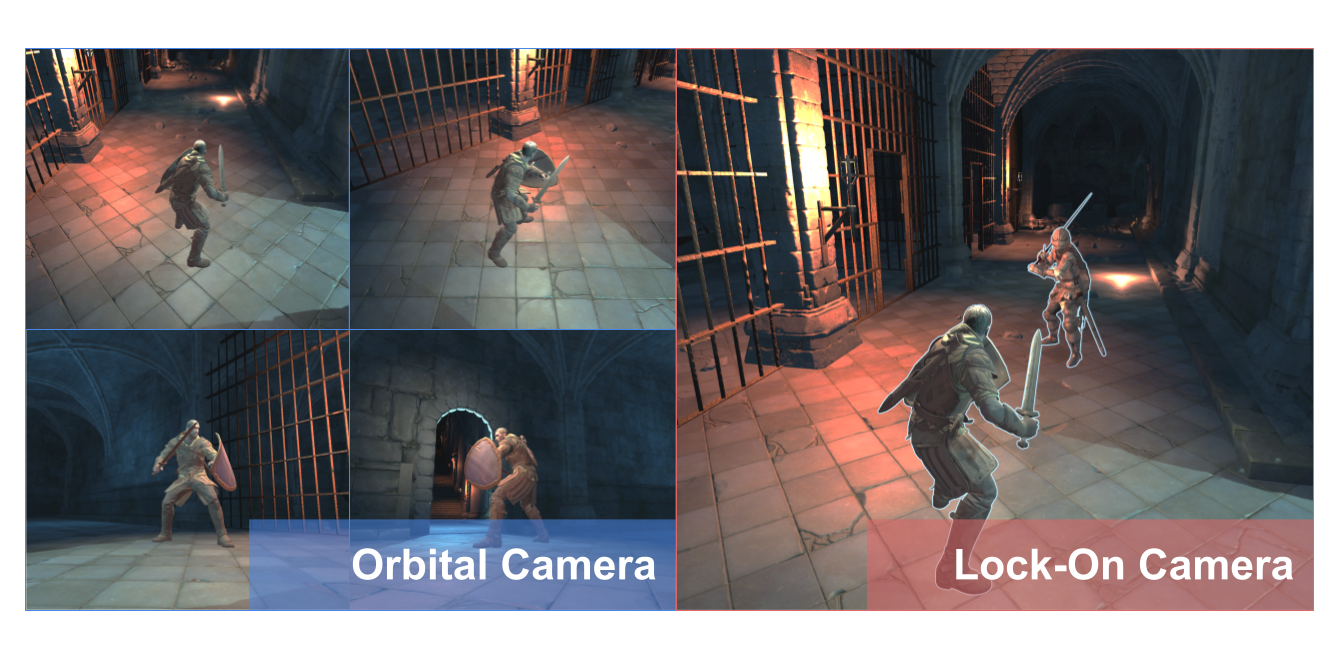
\includegraphics[width=34em]{figures/fig-camera-types.png}
    \end{center}
    \legend{Source: Screen capture of application developed by authors.}
    \label{fig:camera-types}
\end{figure}

% Third Person Orbital Camera implementation
% - Use of Cinemachine
%     - Ready-to use implementation of orbital rotation with parametric spline curve for vertical axis
%     - Smooth transition between virtual cameras which was useful for Orbital Camera and Lock-on modes
Regarding the implementation of the Orbital Camera, we chose to use the \emph{Cinemachine} Unity Package due to its comprehensive API and rich functionality. Cinemachine contains pre-defined implementations for multiple types of cameras, including specific algorithms to manipulate Orbital Cameras. Another useful trait is that the APIs provided by Cinemachine enable defining parametric curves for camera positioning, which reduced development iteration time.

%     - Algorithmic motion that can simulate cinematic behavior with camera shake effect and framing corrections
Cinemachine can also manage, compose and blend between camera shots. We configured camera transitions which were triggered by a signal system, resembling the commonly used \emph{Observer design pattern}\sepfootnote{fn:observer-pattern}. Cinemachine also includes algorithms for procedural motion generation, which were used to generate screen shake effects when the player is attacked by an enemy, and to properly adjust framing when the camera needs to track movement of high velocity targets.

\sepfootnotecontent{fn:cinemachine-brain}{The \textsc{CinemachineBrain} component is responsible for defining the current active camera, camera transitions and the signals that trigger each transition.}

\sepfootnotecontent{fn:unity-main-camera}{The Main Camera is a special \textsc{GameObject} with a \textsc{Camera} component which is responsible for rendering the final output of our camera management system.}

% Prefab GameObject hierarchy with CinemachineBrain at root 
% MainCamera object as a child of the CinemachineBrain
To configure Cinemachine for use in our application, we created a \textsc{Prefab}\sepfootnote{fn:unity-prefabs} with a \textsc{CinemachineBrain}\sepfootnote{fn:cinemachine-brain} component at the root  \textsc{GameObject}\sepfootnote{fn:unity-gameobjects}, and multiple \textsc{VirtualCameras} as child objects. The \textsc{CinemachineBrain} brain component  referenced a \emph{Main Camera}\sepfootnote{fn:unity-main-camera}, which was added the \emph{MainCamera} object as a child of the root.

\sepfootnotecontent{fn:cinemachine-virtual-cameras}{VirtualCameras are Cinemachine abstractions that define the physical properties of a camera along with transposing and composing strategies}

% VirtualCamera child objects that contain definitions for transposing and composing strategies
We also included a set of \textsc{VirtualCameras}\sepfootnote{fn:cinemachine-virtual-cameras} as child GameObjects of the Prefab root. Each VirtualCamera in the hierarchy represents one of the camera modes in our implementation. To implement the position and framing of the Orbital Camera, we set the \emph{Transposing Strategy} property value to Orbital, and we assigned a a pivot point above the player as a LookAt target. For the Lock-On camera, we used the Follow transposing strategy and the Group Composition strategy to frame both the player character and their target enemy.

% PlayerCameraDirector component, which is responsible for receiving signals from player and translating them into signals for the CinemachineBrain and activating and deactivating PlayerCameraBehaviours
We also added a \textsc{GameObject} containing a \textsc{PlayerCameraDirector} component, which is responsible for receiving signals from the \emph{Player} component and translating them into signals for the \textsc{CinemachineBrain}. The signals are then used to switch and transition between shots. The \textsc{PlayerCameraDirector} is also responsible for enabling and disabling \textsc{PlayerCameraBehaviour} components, which receive player input, manage camera framing targets and initialize camera states.

The \textsc{VirtualCamera} components receive player input and process such input into positional or state change actions. For instance, the \textsc{OrbitalCamera} receives a two-dimensional vector as input, which is translated into rotations and translations over the X and Y axes. In the Lock-On camera, the horizontal axis of the vector input is used to switch Lock-On targets. Figure \ref{fig:camera-class-diagram} shows an overview of the class relationship in our camera system implementation, as well as the signals that are being sent and listened to.

% * Figure:  Camera system class diagram
\begin{figure}[!ht]
    \begin{center}
    \caption{A diagram showing the class relationship of our Camera System implementation, along with the signals being sent and processed.}
    \vspace{0.5em}
        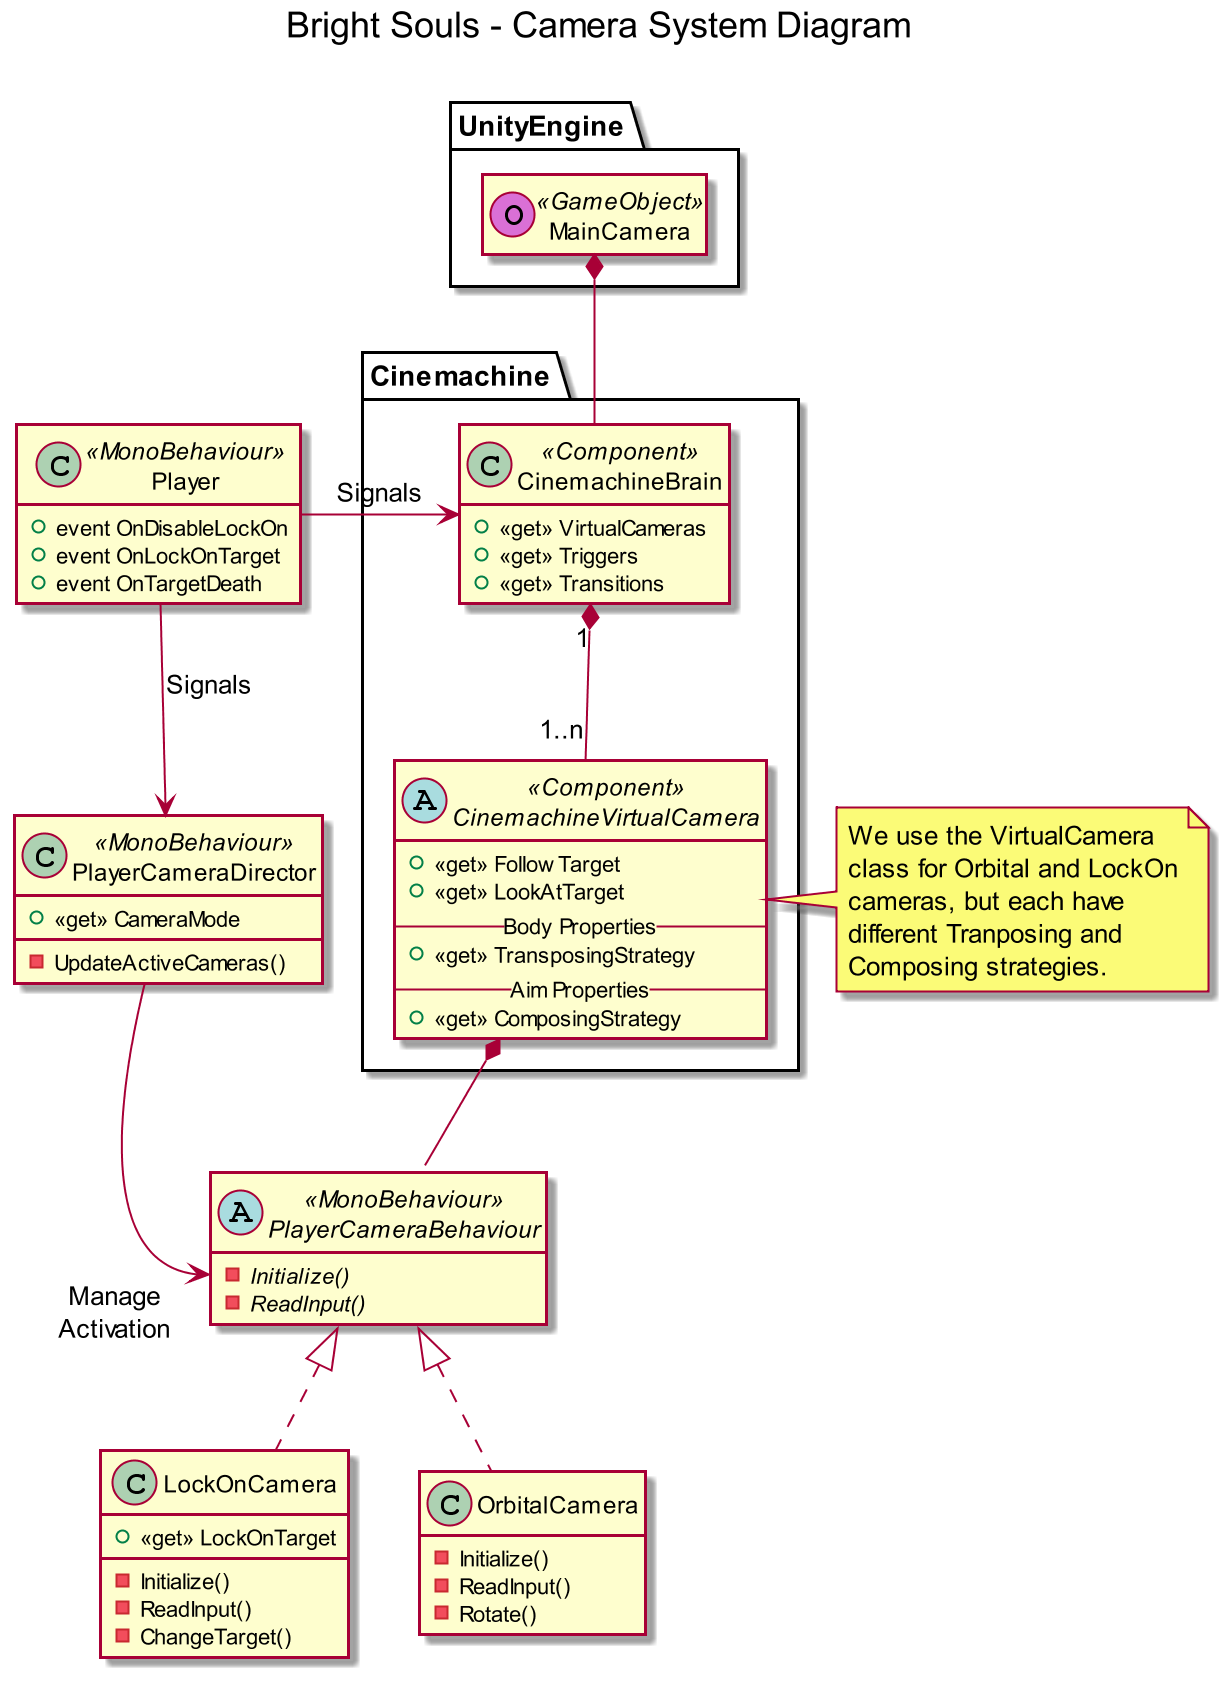
\includegraphics[width=34em]{figures/fig-camera-system-class-diagram.png}
        \legend{Source: Diagram assembled by the authors.}
        \label{fig:camera-class-diagram}
    \end{center}
\end{figure}

%     - Simplified collision geometry enables using a pull-forward collision resolution
To constrain cameras inside the playable space, we used invisible collider objects which define positional boundaries for cameras. Such colliders represent a simplified version of the environmental geometry, using mostly Axis-Aligned Bounding Boxes as intersection validation targets. We use such method to improve the performance of intersection-checking raycasts and to avoid jittery movement when using pull-forward camera collision resolution on thin objects. The invisible colliders are limited to interact with camera algorithms, and do not interact with player movement or any physics entities.

% Lock-On camera and targeting system
% - Possible Lock-on targets must be located in an intersection of the camera viewport with a collision sphere centered at player character
% - Lock-On target prioritization is higher for targets that are closer to the player and to the center of the screen
To detect entities which are eligible to be targets for the Lock-On camera, we use a spheric collider in a radius around the player and check for intersections inside its area. Detected entities inside the spheric collider are intersected with the group of entities which can be seen in the camera's viewport, to constrain Lock-On selection to entities which can be seen by the player. Eligible targets are collected into a list ordered by distance to the player character, which is updated every second. This is done because targets that are closer to the player are considered a higher threat, as they are more likely to hit the player when attacking.

% - Use of horizontal input axis from Orbital Camera to switch between targets
Horizontal player input is used to switch between targets in the Lock-On camera. Moving the input axis to the left switches to the closest target at the left of the current Locked-On target, using coordinates relative to the camera's viewport space. Similarly, moving the input axis to the right will select an entity to the right of the current target. Therefore, the position of the next target is selected by comparing the X axis of entities when converting their coordinates to a camera's viewport space.

% ========================================================================
% ========================================================================
% ========================================================================


% Movement mechanics and physics
\subsection{Movement mechanics and physics}

% Movement in games is not realistic for responsiveness
Traditionally, the movement for player-controlled characters in games is not designed to be physically realistic. Characters will often move at abnormally high speeds, are able to stop almost immediately and can turn their movement direction with ease. This is done so that character movement is highly responsive to raw player input and becomes easier to manipulate in comparison to physics-based controls. If player characters in video games were to be physically accurate, they would take significant time to accelerate to their maximum movement speed and decelerate until stopped, while also having difficulty turning sharp angles at high speeds.

% Characters with physics controls are difficult to control
% Movement physics should be simplified for learn ease
When considering gameplay aspects, characters implemented with physical accuracy feel heavy and difficult to control, forcing the player to calculate the physical properties of their characters and virtual environment. This causes a significant amount of overhead for players desiring to achieve proficiency with motion controls. Therefore, character movement should be a streamlined and trivial mechanic that can be quickly mastered, unless movement itself is a purposefully designed game challenge, such as in \emph{Death Stranding}\sepfootnote{fn:death-stranding}.

% CharacterController for wall and obstacle collision and running over slopes
Considering the need for responsive movement that can be easily mastered, we use the \emph{CharacterController}\sepfootnote{fn:character-controller} component that is natively built-in as part of \textsc{Unity}'s base functionality. CharacterControllers are not affected by native physics systems, and implement common gameplay-related functionality such as the ability to slide along walls when moving in a non-orthogonal angle, detecting and stepping over small vertical offsets in ground geometry such as steps and ledges and handling movement constraints in ramps.

\subsubsection{Camera-Based Movement}

% We define movement direction based on camera orientation
In our implementation, movement input generates different motion types depending on camera state. In the \emph{Orbital Camera}, input causes the player to rotate and move towards a direction which is relative to the camera's orientation. To animate the player's character model in such state, the movement system signalizes a continuous frontal movement to the Animation System. Positional transforms are handled by the Animation System, with the objective of matching movement speed with animation keyframes -- which circumvents \emph{movement drifting}\sepfootnote{fn:movement-drifting} issues.

% We constrain rotation speed for minimal fidelity
A character with minimal physics fidelity should be unable to immediately turn to the opposing movement direction after fully accelerating. However, player controls should still provide some level of responsiveness regarding character rotation changes. Therefore, handling body rotation through player input requires imposing constraints, as it is necessary to create a minimal sense of weight to a character while maintaining an acceptable input response. Thus, the \emph{maximum rotation speed} attribute is implemented to constrain the speed at which a player is able to turn.

% In Lock-On player moves in a circle around enemy
In the \emph{Lock-On}\sepfootnote{fn:lock-on} camera, player input causes their character to move without changing body rotation. In this state, the player character always faces their target. As for the movement direction, the Animation System uses player input to blend movement between three states: forward movement, side steps and back steps. Since the viewport is automatically defined by the positions of the player and their target without considering player input, the player always performs circular movements around their target in the Lock-On state. Camera positioning for \emph{Locked-On Cameras} is further explained in subsection \ref{sec:lock-on-camera}.

\subsubsection{Grounded State Detection}

% Players are unable to accelerate on air
% Gravity vector force applied every fixed step when on air
Another state that was considered in our movement implementation is when the player is not touching the ground, such as when falling from a ledge. In this state, the Capsule-shaped \emph{collider}\sepfootnote{fn:colliders} defined by the player's CharacterController does not \emph{overlap}\sepfootnote{fn:collider-overlapping} with ground geometry. In such situation, the player character should be considered "On-Air", and movement input should have less influence in motion. Should the player's character be able to accelerate, decelerate or turn while airborne, players might experience a break in the immersion. In our implementation, we constantly accelerate our CharacterController velocity by a gravity vector on fixed time steps when the player is not on ground.

% Gravity and grounded state detection: use of SphereCast
To detect if the player is airborne, we perform a collider intersection check between the player and ground geometry. We make use of \emph{Unity's} built-in \emph{SphereCast} operation, which  performs multiple sequential intersection checks of a sphere envelope (a spheric collider with a radius slightly higher than the player's character model radius) with ground colliders. The intersection checks are performed along a \emph{Ray}\sepfootnote{fn:rays}, which originates from the center of the player's character model and extends along the gravity vector. We use a length of three quarters of the player's collider size as a distance limit to detect the ground. 

% High vertical speed, stuck in geometry
With the use of rays for collision detection, vertical collisions can be detected ahead of time when the player is falling at high speeds. This circumvents the common problem in video game physics where when the player's vertical speed is too high, they could become stuck inside ground geometry if the collision detection algorithm does not take into account the game's update rate. Another advantage of using \emph{Raycast-type}\sepfootnote{fn:raycasts} operations is precisely detecting the points where a collider intersects with a ray. This enables precise definition of which parts of a collider interact with ground geometry. Listing \ref{lst:grounded-detection} shows our implementation for detecting ground collision. % TODO add footnote for this

\begin{lstlisting}[caption={Implementation of grounded state detection.},label={lst:grounded-detection}]
var ray = new Ray(transform.position, Vector3.down);
grounded = Physics.SphereCast(ray, charController.radius + 0.1f, charController.height / 2f + 0.5f, physicsData.GroundDetectionLayers.value);
// Animator also applies gravity, so when not grounded disable animator physics
player.Anim.applyRootMotion = grounded;
\end{lstlisting}
\label{lst:ground-detection}

 In contrast to Ray Intersections, the SphereCast operation used in our algorithm is able to detect overlaps in a volume, which means that complex collider setups which intersect in the borders of a Capsule are detected. A common situation in games where platforms and gravity can affect the player is that players might find themselves above multiple close but separated ledges. Raycast operations are unable to handle this situation, as the rays might not intersect with any of the ledges.

% TODO Figure: Example showing visual difference of Raycast vs SphereCast

If grounded-state detection is not handled appropriately, components which handle entity acceleration might accumulate vertical velocity indefinitely. If the player is colliding with ground geometry but the logical systems consider the player On-Air, player velocity constantly accumulates the gravity force. In such cases, after player steps away from a ledge, their character instantly falls to the ground in abnormal speed. If the game is programmed to apply fall damage, this often results in instant death, even though the player did not fall from a considerable height.

In the frame where a character that is On-Air detects ground collision, we invoke the \textsc{OnHitGround} event, and proceed to perform fall damage calculation. In our implementation, fall damage is calculated by considering fall speed multiplied by a parametrized speed-to-health-point conversion factor, named 'FallDamageMultiplier'.

\subsubsection{Movement System Design}

Figure \ref{fig:movement-class-diagram} shows an overview of the class architecture for our implementation of the movement system. We implement top-level \textsc{Player} class which contains the components for all gameplay-related subsystems. The \textsc{PlayerMotor} component is an implementation of the \textsc{ICharacterMotor} interface, and is responsible for implementing the movement and physics logic of our motion controls.

When input is received from the user, the \textsc{PlayerMotor} component filters the input, calculates a target movement direction based on viewport orientation, and delegates position changing to the \textsc{Player.Move()} method. The \textsc{Player} class calls the \textsc{CharacterController.Move()} method from Unity's API, which considers collisions and other physics-related constraints. The \text{Player.Move()} method also broadcasts animation-related signals that are consumed by the \textsc{PlayerBody} class, which in turn communicates with Unity's \textsc{Animator}.

% Figure: Player Movement Class Diagram for Bright Souls
\begin{figure}[!ht]
    \begin{center}
    \caption{Class diagram representing the architecture of our Movement System.}
    \vspace{0.5em}
        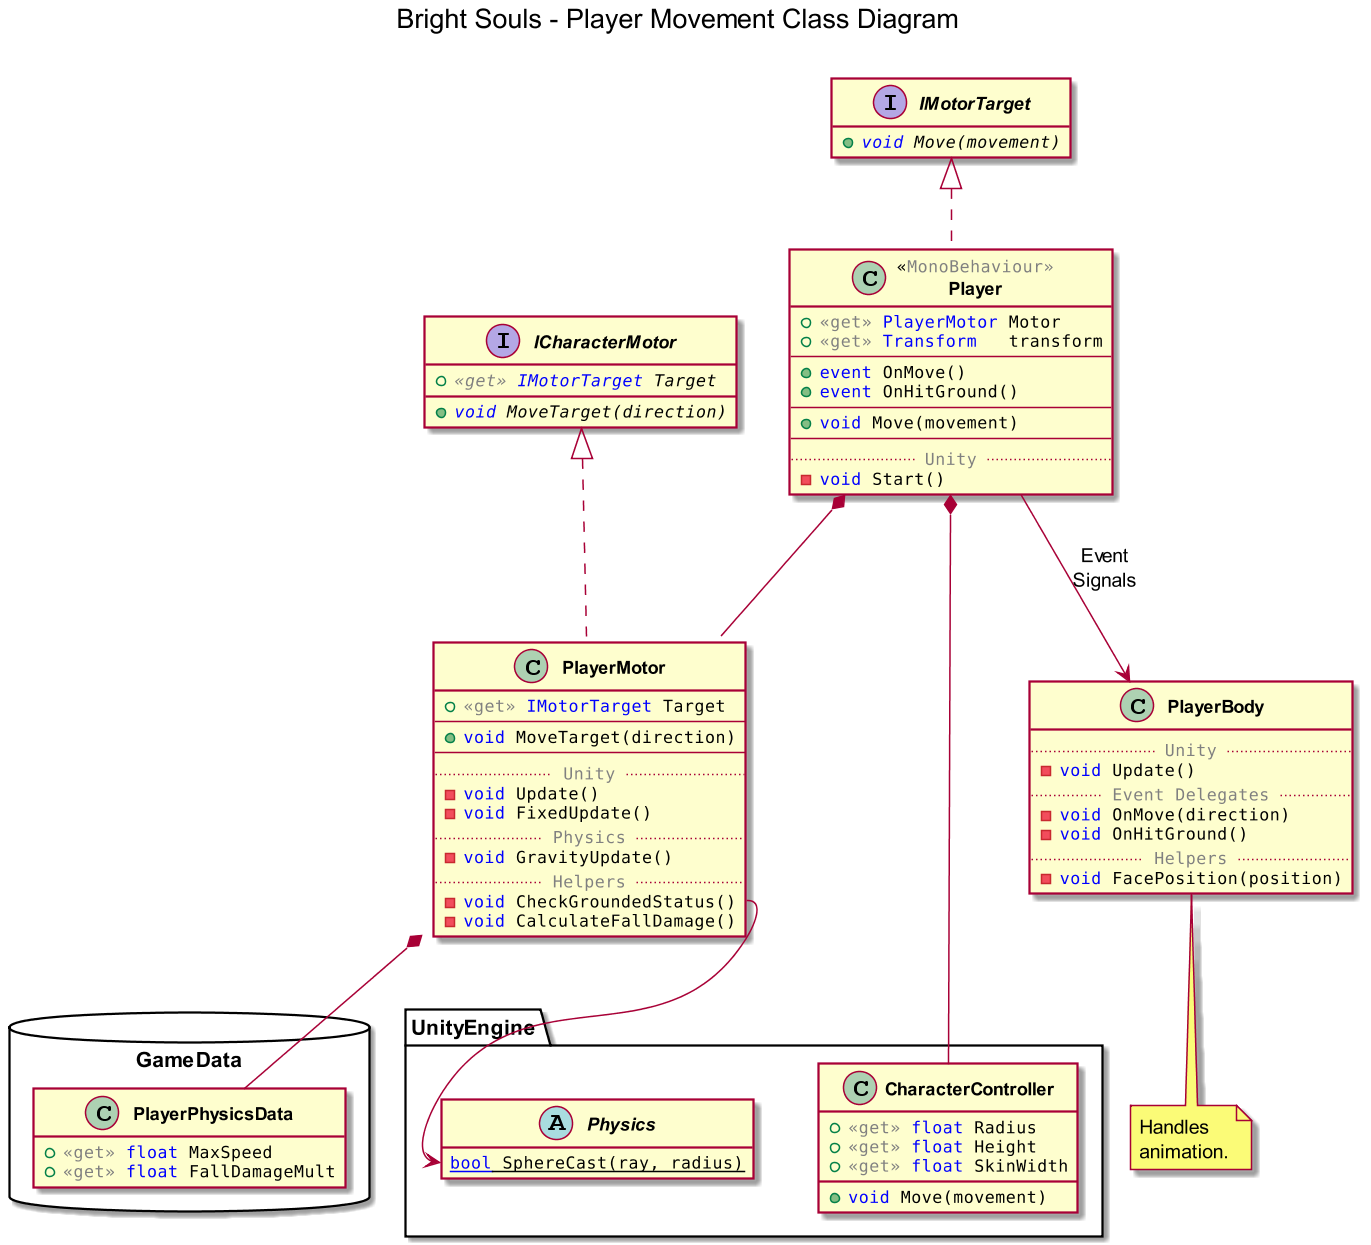
\includegraphics[width=34em]{figures/fig-player-movement-class-diagram.png}
        \legend{Source: Diagram assembled by authors.}
        \label{fig:movement-class-diagram}
    \end{center}
\end{figure}

% ========================================================================
% ========================================================================
% ========================================================================

\subsection{Attributes System}

% Attributes system
In our implementation, we define an abstraction layer for runtime variables that represent the state of game entities, and can be serialized through saving and loading. Attributes are used to represent status for the Player and enemies -- with variables representing health, stamina, poise, damage, speed and others. We also use attributes to define the state of interactable objects such as doors and levers -- with boolean variables such as \textsc{isOpen} or \textsc{isToggled}. Attributes can be initialized, serialized and monitored by external systems, such as the native dependency injection in Unity's \textsc{Inspector} and our data persistence system which serializes runtime data through scenes.

% Based on Generics: Attributes can be generated for any primitive type, such as int, float, double, string.
%   - Serialized into binary gameplay data files for game designers to define the default and maximum values for character health, stamina and poise
%   - Initialized by persistent data managers to maintain player status when transitioning between levels
Attributes are based on \textsc{C\#} \emph{Generics}, and can be generated for any value type such as integers, floating point variables, strings and enumerations. This limitation is imposed in our architecture so that attributes can be easily serialized into binary data files that can be used to define the default and maximum values for each attribute holder. This constraint also facilitates Attribute initialization, which is useful to support persistent data such as maintaining attributes between levels  or loading the state of an entity from a file in a savegame system.

\sepfootnotecontent{fn:ui-health-bars}{Health bars show the current player health and also provide a good estimation of health lost when getting attacked by an enemy using a secondary, trailing health bar.}

%   - Monitored by UI systems to display relevant data about the status of the player, for instance a Health Bar that display the current health of the player and shows health lost when getting attacked.
Attribute specializations implement the \textsc{IAttribute} interface, which exposes acessors for data manipulation and events for value changes. Events facilitate the use of attributes by external components, decoupling independent systems in our architecture. An example can be observed in our UI (User Interface) elements, which subscribe to value change events in player status attributes such as Health, and update Health bars\sepfootnote{fn:ui-health-bars} whenever the health attribute publishes a change.

Another advantage of using event systems is the flexibility to add and remove subscribers as required. As an example, when implementing the UI for the player character we can initially propose a single health bar to monitor player health. If requirements for our application change, we can iteratively add new elements such as floating text, combat messages and visual effects without prior knowledge of which systems will be required in the final release. 

% - AttributesContainers
%     - Containerization of attributes to allow for entities with different attribute configurations without defining static types
%     - Possibility to dynamically assign attributes during the course of a session, which can be useful for a telemetry system
% - Definition of interfaces that expose attributes to any of the classes that might require it
To decouple attributes from their owners and the systems which modify them, we created a standardized interface for containerizing and accessing them under different entities. We implement \emph{Attribute Containers}, which provide a public interface for instantiation, access and manipulation of statically typed attributes for an entity. Attribute Containers can be queried by external systems for type-based compatibility. By using this access layer, we can provide polymorphic attribute mutability based on compatibility. Figure \ref{fig:attributes-diagram} shows an overview of the class relationships in the Attributes System, along with examples of how attributes signalize changes to external components such as UI Elements.

% * Figure: Attributes system class diagram
\begin{figure}[!ht]
    \begin{center}
    \caption{Class diagram for the Attributes System, showing examples of signals being used by UI Elements.}
    \vspace{0.5em}
        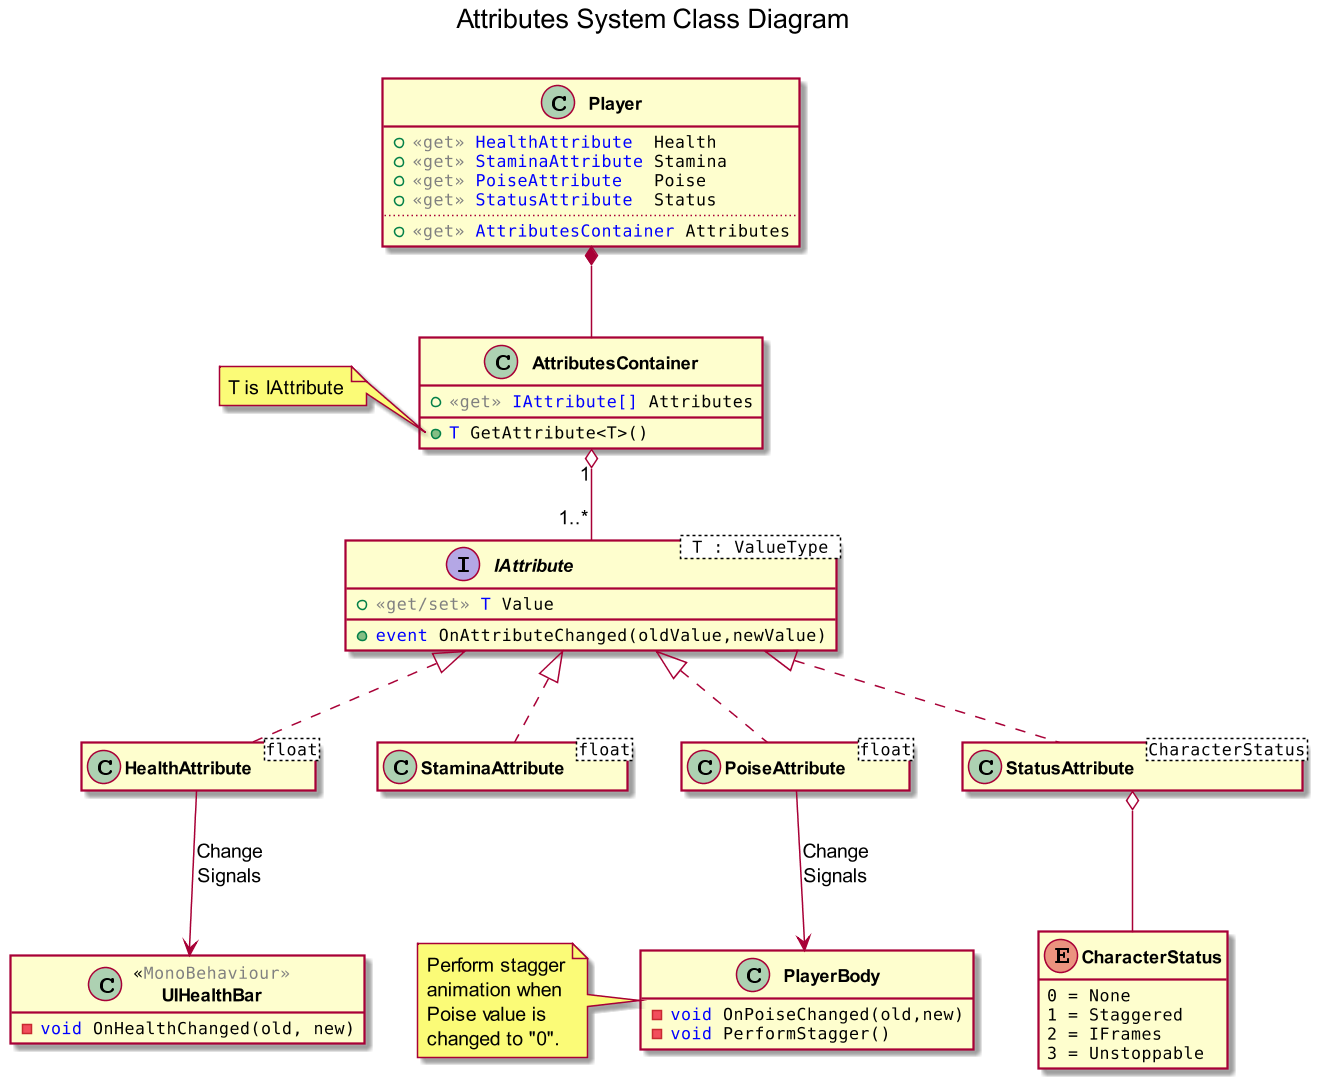
\includegraphics[width=34em]{figures/fig-attributes-diagram.png}
        \legend{Source: Diagram assembled by the authors.}
        \label{fig:attributes-diagram}
    \end{center}
\end{figure}

% ============================================================================
% ============================================================================
% ============================================================================

\subsection{Combat System}

% Combat System involves:
% - Managing attacking and combo animation and logical states for the player
% - Being able to detect when the weapon of the attacker collides with a target
% - Being able to detect when the target was able to block or dodge an attack
% - Applying combat effects when the target is hit
To implement the combat mechanics in our \emph{Souls-like} implementation, we defined a list of requirements for combat-related components:
\begin{itemize}
    \item{Manage attack animations and logical states for the player character;}
    \item{A \emph{Hit Detection System} which is able to detect when the weapon of the attacker overlaps with the \emph{Hitbox} of a target to validate a \emph{Succesful Hit};}
    \item{Verify if attacks are blocked or dodged, and apply modifiers to Combat Effects;}
    \item{Apply \emph{Combat Effects} when a target is hit, such as a \emph{Health Damage} effect;}
    \item{Modify character state according to the effects that are applied.}
\end{itemize}
By invoking the aforementioned functionality with player input and AI agent actions, we created a satisfactory combat system that provides appropriate feedback to player actions and decisions. In figure \ref{fig:combat-system-overview}, we provide an overview of the subsystems and classes regarding to our implementation of a Combat System.

% * Figure: Combat System Overview Diagram
\begin{figure}[!ht]
    \begin{center}
    \caption{A class diagram containing an overview of the class relationships in our Combat System implementation.}
    \vspace{0.5em}
        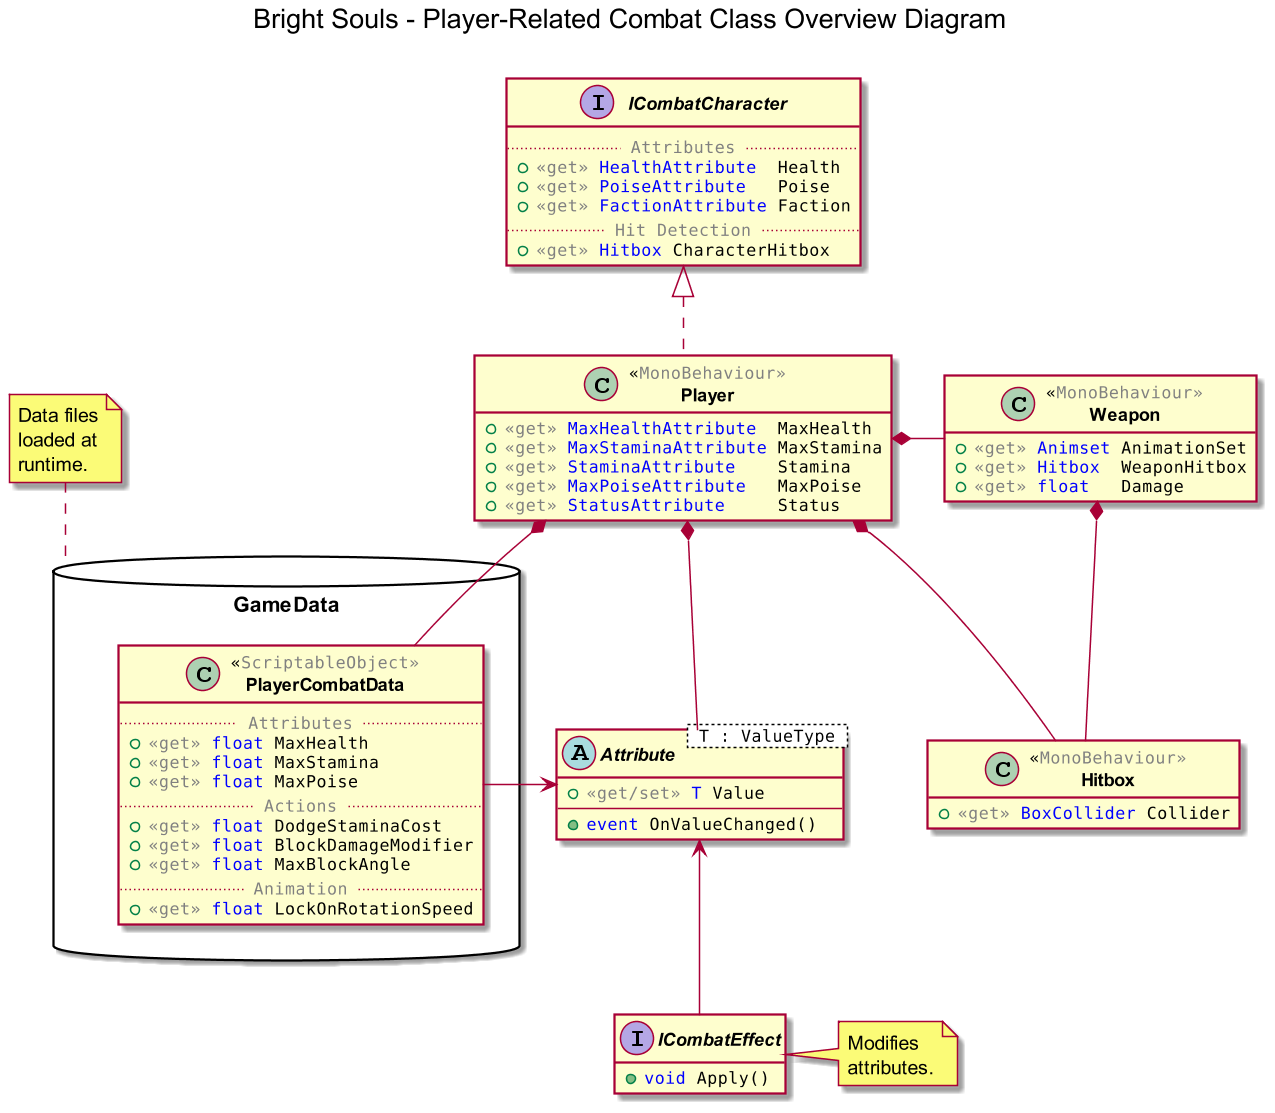
\includegraphics[width=34em]{figures/fig-combat-system-overview.png}
        \legend{Source: Diagram assembled by authors.}
    \end{center}
    \label{fig:combat-system-overview}
\end{figure}

\sepfootnotecontent{fn:command-pattern}{\emph{Command} is a commonly used code design pattern to encapsulate data and actions related to an event into an object. In games, the Command pattern is commonly used as a layer of separation between the Input system and the response triggered by input in in-game entities.}

\sepfootnotecontent{fn:current-player-state}{The current state of the player is defined by a composition of boolean variables that reflect by the Animation being played on their character model.}

% Attacking and combo system
%  - Continuously check for Attack input
The entry point for our combat system is invoking, either through player input or AI issued commands, of combat-related \emph{Commands}\sepfootnote{fn:command-pattern}. We defined a dictionary-based data structure to map input button codes to player character commands. The keys to our dictionary are queried for at every frame, and if a key press is detected we execute the command which represents its respective value. For instance, if the button mapped to the \emph{Attack Command} is pressed, we proceed to verify the current state\sepfootnote{fn:current-player-state} of the player to determine if an attack can be performed.

% - Player/character is unable to perform attack if on Animation Lock
% - Attacks cost Stamina
For each Command, we define a set of restrictions which block the player from executing such command if their validation condition returns false. For instance, in our implementation the player is unable to attack if they are executing an action which would render their character unable to use their sword. Therefore, if the player is in the \emph{Dead}, \emph{Staggered}, \emph{AttackEnding}, \emph{On-Air}, \emph{Landing}, \emph{Dodging} or \emph{Blocking} states, they are considered unable to perform an attack, and thus the validation for the \textsc{IsNotBlockedByAnimation} restriction fails. This is commonly referred to as \emph{Animation Locking} in games, and is considered a crucial feature used to balance game difficulty. Attack Commands also have a resource cost for the player, where each attack depletes an amount of \emph{Stamina}. If the player Stamina resource has a value of zero, the player is unable to perform an attack. Therefore, we also define the \textsc{HasStamina} restriction, requiring the value of the player's \emph{Stamina} attribute to be higher than zero.

%  - When sending attack command, enter a "combo" state and "Attack animation state machine"
%  - "OnCombo" state:
%    - Preemptively read player input before current attack animation ends. If player successfully sent attack input, continue the combo.
%    - If no attack input command is read within animation time frame, escape the Attack animation state machine
After an Attack Command is successfully validated, the player's state is set to \emph{Attacking}. An \emph{Attack State Machine} is initiated, where Attack Commands are preemptively checked for during attack animations. If an Attack Command is successfully executed before an attack animation ends, an \emph{Attack Chain} is toggled, causing the next attack animation to be queued and triggered when the current animation ends. This behavior is commonly referred to as a \emph{Combo} in video games. If no Attack Command is successfully executed within the \emph{Attack Chain} time frame, the player exits the \emph{Attack State Machine} and is locked to a short \emph{AttackEnding} animation state. Figure \ref{fig:player-anim-state-machine} shows the state machine used to implement the aforementioned behavior.

% Figure: Player Animation state machine
\begin{figure}[!ht]
    \caption{A state machine used for our implementation of the Attack and Combo system.}
    \vspace{0.5em}
    \begin{center}
        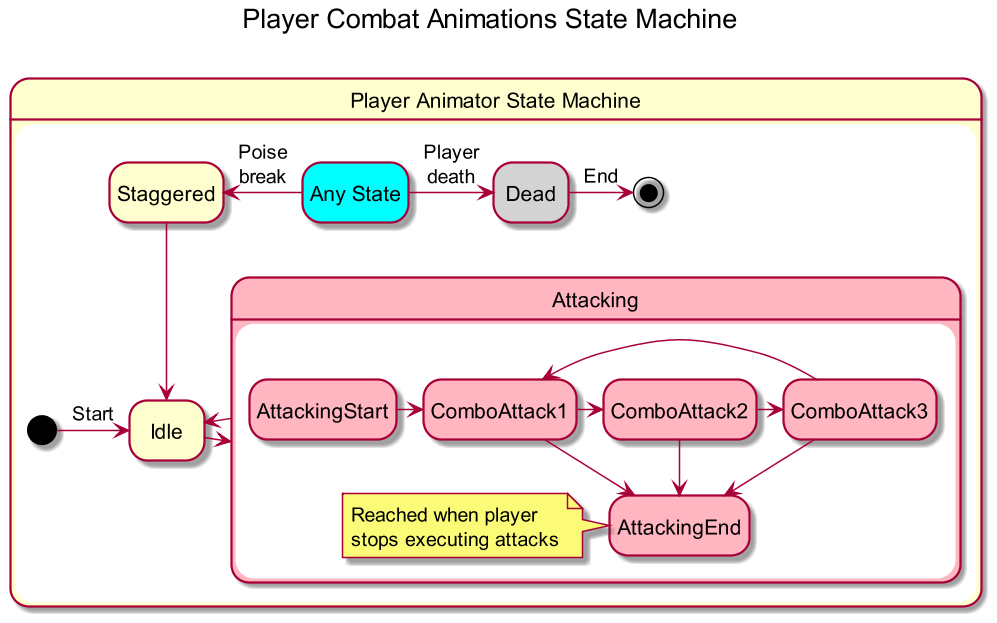
\includegraphics[width=34em]{figures/fig-player-anim-state-machine.png}
    \end{center}
    \legend{Source: Diagram assembled by authors.}
    \label{fig:player-anim-state-machine}
\end{figure}

\sepfootnotecontent{fn:attack-collision-end}{The \textsc{AttackCollisionEndEvent} is required to be signalized after the \textsc{AttackCollisionStartEvent} and before the attack animation ends so that attacks appropriately reflect what the attacking character performs.}

%   > Hit detection toggled when receiving an event signal from the Attack animation
During combat-related animations, the Animation System broadcasts event signals that toggle the activation or deactivation of the \emph{Hit Detection System}, which has the purpose of validating whether an attack successfully hit an enemy. At a certain point during the attack animation, we broadcast the \textsc{AttackCollisionStartEvent}, which signalizes that attack collisions must be checked on each frame until the \textsc{AttackCollisionEndEvent} is published. The \textsc{AttackCollisionStart} and \textsc{AttackCollisionEnd}\sepfootnote{fn:attack-collision-end} events are triggered in the short time frame where a character swings their weapon. Figure \ref{fig:attack-combo-diagram} shows the relationships between components involved in issuing Attack commands and handling hit detection.

% Figure: Attack and combos Class Diagram
\begin{figure}[!ht]
    \begin{center}
    \caption{A diagram showing the event flow and class relationship of the Attack and Combo related classes.}
    \vspace{0.5em}
        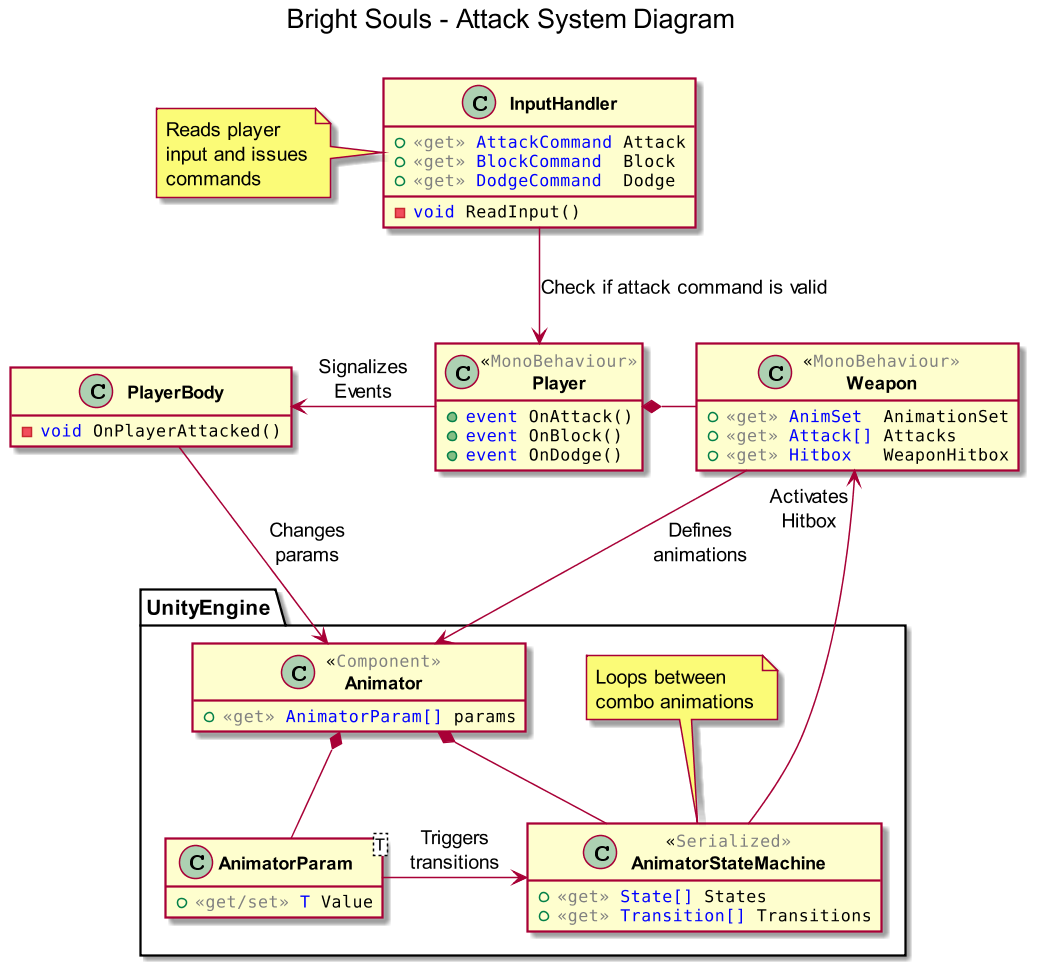
\includegraphics[width=34em]{figures/fig-attack-combo-diagram.png}
        \legend{Source: Diagram assembled by the authors.}
    \end{center}
    \label{fig:attack-combo-diagram}
\end{figure}

%     - Hit detection must not occur twice between the same target and same attack
%     - Specific collision layer to detect hitbox collision
To implement hit detection, we perform collision intersection checks in fixed time intervals of 16 milliseconds. Objects involved in combat-related collision checking are restricted to a special layer called HitDetection, where every Collider is either the weapon of an attacker or the body of a target. Restricting the elements involved in a hit detection system is a required optimization for collisions to be detected consistently. If the Hit Detection system is unable to meet the 16 milliseconds time constraint, there is a small chance that an attack might not be detected, where an attacker weapon "passes-by" the body of the attacker without triggering the collision event.

We estimate that in our implementation attack collision detection occurs for approximately 20 frames from the point where it is first activated. Thus, if a computer system is able perform at least 4 updates per second, attack collision is guaranteed to be correctly detected. It is important to note that updates to the collision detection system are independent to the rendering performed by the graphics pipeline, and as a consequence are unaffected by graphics-related stuttering.

We also employed several safety measures to ensure that attack collision detection does not trigger a \emph{Hit} event twice for a same attack input. Therefore, we store a reference to an \emph{AttackCollision} instance in the \emph{Hitbox} component of the target entity for each attack command. The Hitbox component listens for the \emph{AttackCollisionEndEvent}, which determinesn when the reference can be deleted. At this point, the attacker's hit detection system does not perform any collision checks for the same attack.

% - Hit detection:
%   > Colliders:
%     - Hitbox overlap detection for attacker weapons and target character
%     - Attack Colliders are bounding boxes in weapons
%     - Character colliders are simplified bounding boxes that enclose torso, head and partially legs
For each occurrence of an attack collision, two colliders are involved: one for the weapon of the attacker, and one for the body of the target. The colliders are instanced as \emph{bounding boxes}\sepfootnote{fn:bounding-boxes} that fully or partially enclose the 3D models of their relative entity (an attacker's weapon or a target's body). To perform collision checks with a reasonably optimized numbers of collision checks, we simplify collision by introducing a single bounding box that encloses the torso, the head and a central position of the target's legs. Using this method, we minimize the amount of collision checks per frame, while also having appropriate precision for our gameplay purposes.

%     - Consider character faction to recognize which combat characters can be hurt by an attack
After the collision detection step is performed, we validate that the target is not part of the attacker's \emph{Combat Group} by comparing the \textsc{FactionAttribute} value of the involved entities. We perform such distinction to avoid a situation where player enemies would damage themselves when attempting to hit the player when too close to each other. The values that the faction attribute can be assigned are described in table \ref{tab:table-faction-groups}. In addition, figure \ref{fig:hit-detection-diagram} shows the execution flow and class relationship of components used during the Hit Detection step.

% * Table: Values for the Faction Attribute
\begin{table}
    \begin{center}
      \caption{A description of the values that can be assigned to the \emph{Faction Attribute} of targets that are part of the Combat System in our implementation.}
      \label{tab:table-faction-groups}
      \rowcolors{2}{}{gray!25} % Alternate row colors
      \begin{tabular}{ >{\small}w{l}{3em} >{\small}w{c}{3em} m{25em} } % alignments and column size
        \addlinespace
        \toprule
        % Headings
        \bf Name    & \bf Id   & \bf Description                                              \\
        \midrule
        % 3D Models
        Player       &       0 & Player character. The player is a single entity and the sole 
                                 participant of this faction group.                           \\

        Enemy        &       1 & AI Agents that represent Enemies, which are hostile to the 
                                 player character.                                            \\

        NPC          &       2 & Non-Playable Characters. AI Agents which are not hostile to 
                                 the player character, but are hittable by and potentially 
                                 hostile to Enemies. An example of a Non-Playable Character 
                                 would be a companion which follows the player character and 
                                 aids them in combat encounters, being hostile to characters 
                                 belonging to the Enemy faction.                              \\

        Interactable &       3 & Static objects that can be attacked by the Player, Enemies or 
                                 Non-Player Characters and provide some type of feedback when 
                                 attacked. An example of an interactable entity would be a 
                                 barrel that can be attacked and destroyed.                   \\
        \bottomrule
      \end{tabular}
    \end{center}
\end{table}

% * Figure: Hit detection class diagram
\begin{figure}[!ht]
    \begin{center}
    \caption{Class diagram showing an overview of the components and flow of events related to the \emph{Hit Detection System}.}
    \vspace{0.5em}
        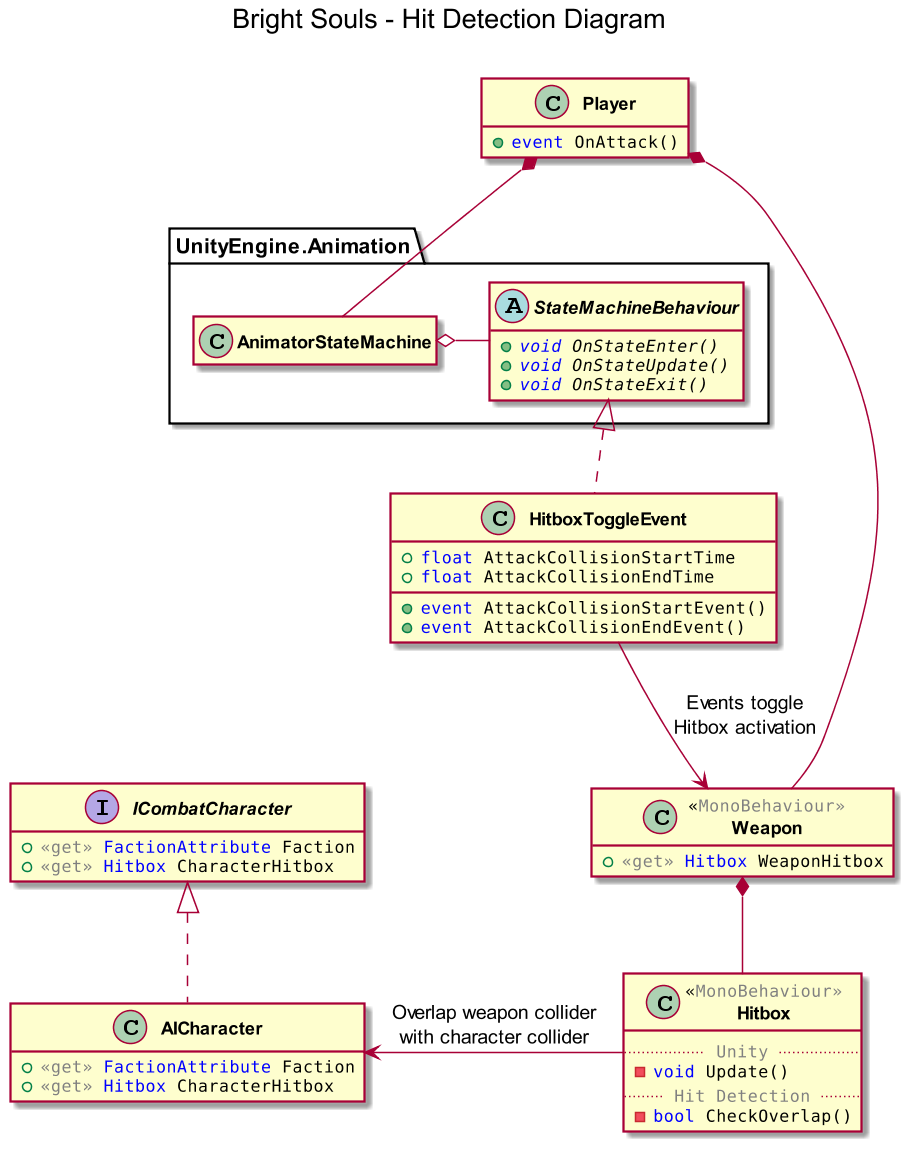
\includegraphics[width=30em]{figures/fig-hit-detection-diagram.png}
        \legend{Source: Diagram assembled by authors.}
    \end{center}
    \label{fig:hit-detection-diagram}
\end{figure}

% - Attack damage and other effects are abstracted into Combat effects
%     - Manipulate character attributes, statuses and physics
After validating an attack as a \emph{Succesful Hit} to a target, we apply \emph{Combat Effects} contained by the Attack onto the target. Combat Effects are containers to a set of attribute changes, status changes and any behaviors that might occur when a character is struck by an attack. Examples of Combat Effects include the \emph{Damage} dealt to the Health of a target, a \emph{StatusEffect} such as a \emph{Stagger}\sepfootnote{fn:stagger} and physics effects such as a \emph{Knockback}\sepfootnote{fn:knockback}. To be affected by a combat effect, the target entity must possess a compatible component or attribute which is able to handle the change proposed by the effect. Therefore, if the player hits an entity and applies the \emph{DamageHealth} effect to a target, the target has to possess the \emph{HealthAttribute} component for the effect to be applied. Figure \ref{fig:combat-effects-diagram} shows an overview of the relationship between classes and components regarding the application of \textsc{CombatEffects} to \textsc{ICombatTarget} entities.

% * Figure: Combat Effect class diagram
\begin{figure}[!ht]
    \begin{center}
    \caption{Class diagram representing the relationships for Combat Effects and affected components.}
    \vspace{0.5em}
        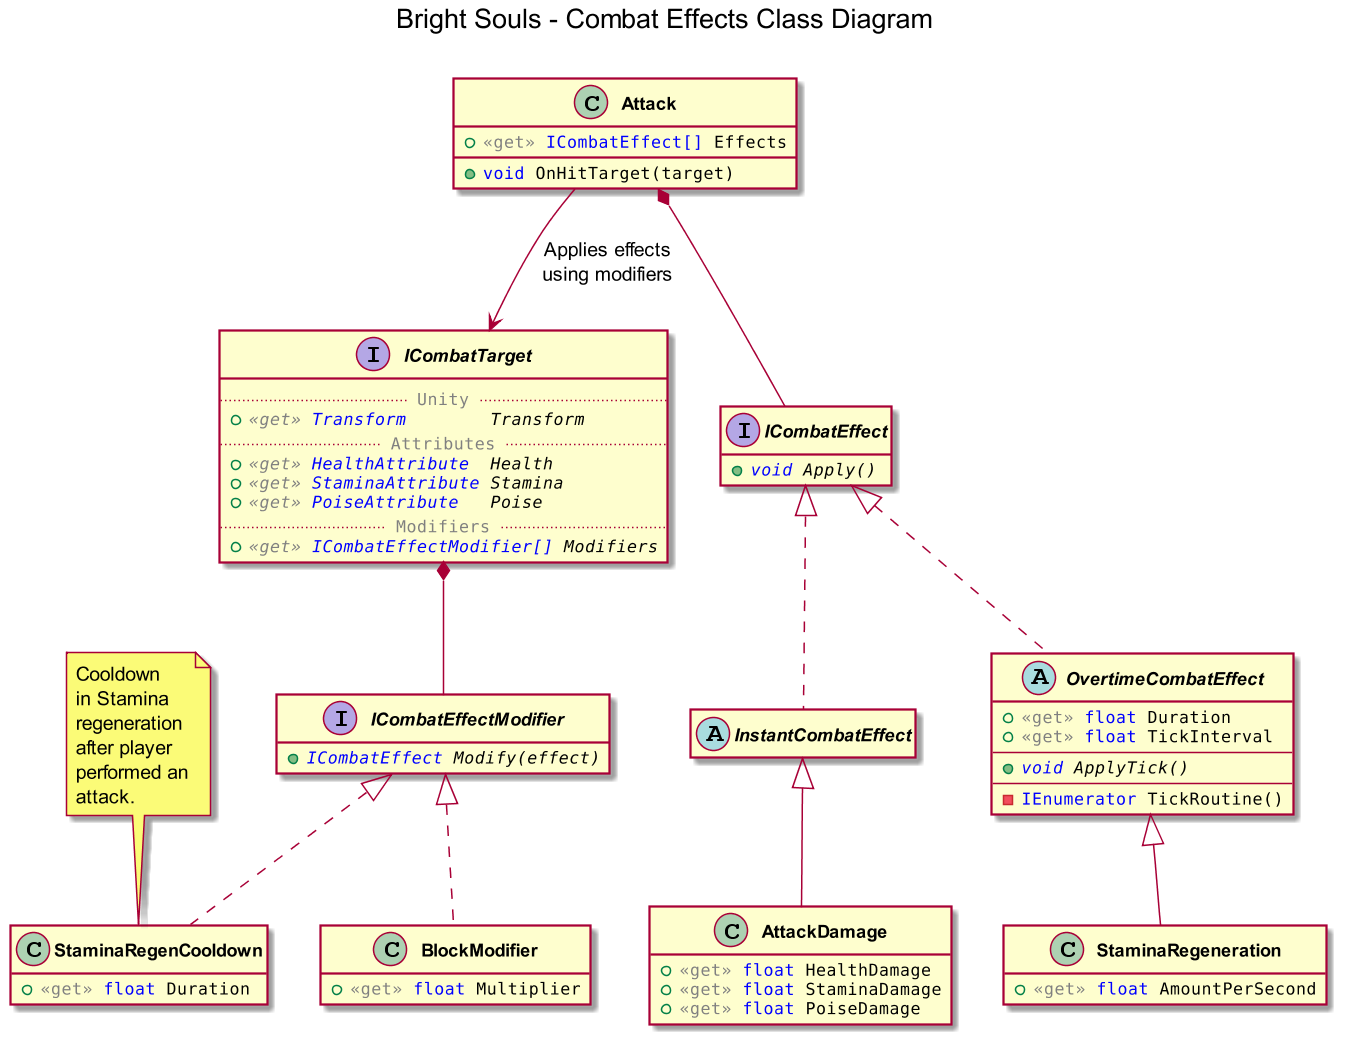
\includegraphics[width=32em]{figures/fig-combat-effects-diagram.png}
        \legend{Source: Diagram assembled by authors.}
        \label{fig:combat-effects-diagram}
    \end{center}
\end{figure}

%     - Instant combat effects are completely applied in the same frame as hit detection occurred
%     - Over-time combat effects with fixed interval ticks
We differentiate between \emph{Instant Combat Effects} and \emph{Over-time Combat Effects}. Instant Effects are applied to a target when a discrete event such as an attack takes place, and simply modify the value of an attribute or apply a temporary \emph{Status}. Examples of Instant Effects include the Health damage caused by an attack, which is applied to the target; And the Stamina cost of performing the attack, which is applied to the attacker. A status change effect can be seen when the player performs the \emph{Dodge} action, which temporarily applies the \emph{Invincible} status effect to their character.

% Player has a default Stamina regeneration effect
In contrast, Over-time Effects occur in fixed time intervals over the course of a duration (or can have an unlimited duration, being bound to the lifetime of an entity). An example of Over-time effect would be \textsc{StaminaRegeneration}, an effect which is permanently applied to the player when not performing any combat-related actions. During the course of a level, the player recovers a fixed amount of Stamina over fixed time intervals. The regeneration is blocked temporarily by the \textsc{StaminaRegenBlock} effect after the player performs any combat-related action which makes use of Stamina, such as attacking, dodging or being struck by an attack. After a certain amount of time without issuing combat-related commands, the \emph{StaminaRegeneration} effect is re-enabled. We also apply modifiers to the amount of recovered stamina under certain circumstances. For instance, entering the Blocking state halves the amount of stamina recovered by applying the \textsc{BlockingStaminaRegenModifier} effect.

% - Combat Effect Modifiers
Combat Effects are restricted to performing modifications on a limited set of Attributes and Components exposed through the \textsc{ICombatTarget} interface, which is implemented by any entity which can be attacked. Before effectively applying an effect to a target, we first check if the target contains any \emph{Combat Effect Modifiers}, such as a damage modifier caused by the target \emph{Blocking} or \emph{Dodging} an attack. If the target has compatible effect modifiers, the \textsc{Attack} class uses such modifiers to reconstruct its Combat Effects with updated values. For instance, if the target successfully blocks an attack, the \textsc{BlockDamage} modifier is applied to any \textsc{DamageHealth} effects by halving the damage amount. After the reconstruction of Combat Effects using any applicable modifiers, we apply the final effect to the target entity.

In figure \ref{fig:combat-flow-diagram}, we show an overview of all the steps involved with handling attacks, starting from the player issuing Attack commands through the Input System, proceeding to the management of animation states associated with weapons, validating Hitbox collision and combat groups with a Hit Detection System, and finally applying combat effects to modify target attributes and execute behaviors.

% * Figure: Flow of Combat System when processing Attack of entities
\begin{figure}[!ht]
    \begin{center}
    \caption{An event flow diagram that shows an overview of each step in our implementation of attacking in the Combat System.}
    \vspace{0.5em}
        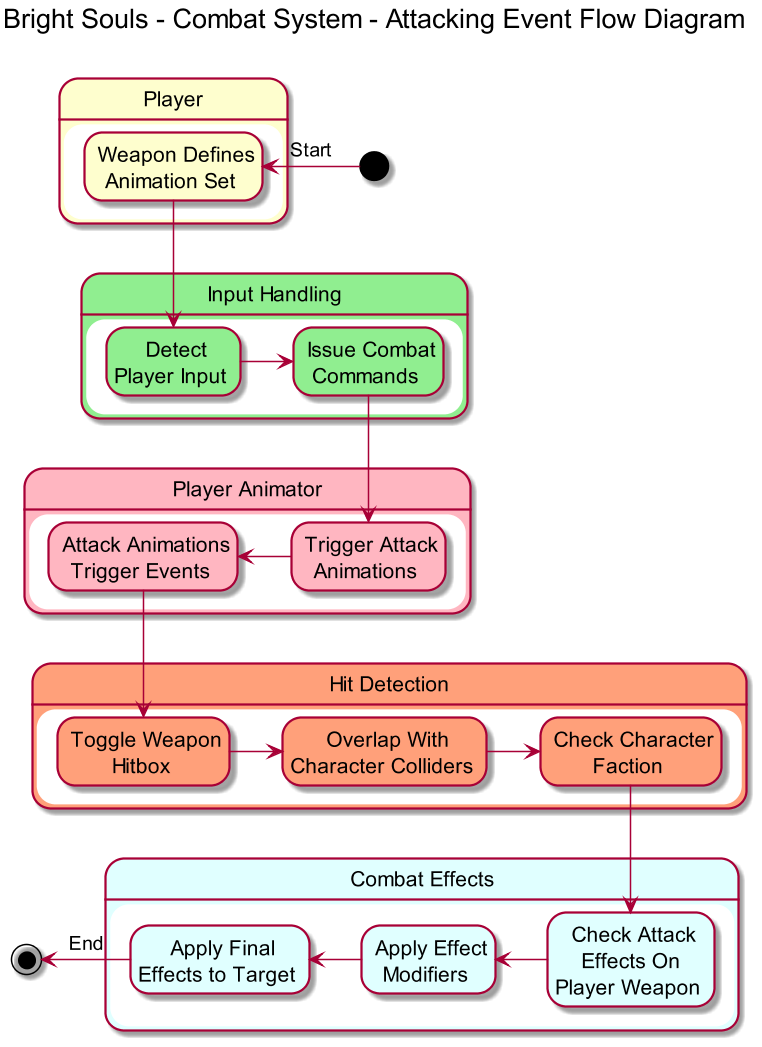
\includegraphics[width=22em]{figures/fig-combat-flow-diagram.png}
        \legend{Source: Diagram assembled by authors.}
    \end{center}
    \label{fig:combat-flow-diagram}
\end{figure}

%     - Block detection occurs when target is hit, is in "blocking" state and vector dot product between attack and target directions is < 0
To perform a \emph{Block}, the player is required to hold an input button which continuously issues the \textsc{BlockCommand}. When the player character is hit by an attack while performing a Block, we calculate the vector dot product between the attacker and player directions to determine if an attack was succesfully blocked. If the result of the dot product has a negative value, the player is considered to be correctly pointing their shield towards the target, which results in a successful block. If the result has a positive value, we consider that the target attacked the player from their flank or back, and thus the player was unable to block the attack.

%     - Dodge detection also occurs when target is hit. If hit detection occurs during target invincibility frames, a "dodge" is registered, and target receives no combat effects
Contrary to blocking, the \textsc{DodgeCommand} is issued at the discrete press of a button. When the dodge command is issued, the \emph{Dodge} action is signalized to the animation system, which in turn responds by moving the player character accordingly. If the dodge command is issued towards a specific direction (by using a movement command), the Animation System translates the character towards such direction. If the player is stationary when issuing the dodge command, the \textsc{Animator} simply uses the current direction being faced by the player character as a translation direction. Over the duration of the dodge animation, we issue the \textsc{DodgeIFramesBegin} and the \textsc{DodgeIFramesEnd} events, which toggle the \textsc{Invincibility} status to the player. Combat invincibility effect nullifies any combat effects towards the player.

% ========================================================================
% ========================================================================
% ========================================================================

% TODO \subsubsection{Animation System (ADDITIONAL)}

% Animation system
% - Difference in body movement when in Orbital vs Lock-On Cameras
% - React to attribute changes, motor velocity and physics updates

% - Figure: Player Animation State Machine

% - Statuses such as staggered, dead will override other animations
% - Blending between animations states when performing directional actions
% - Transitioning between combo states
% - Animation events for hit detection when attacking

% - Figure: Animation System class diagram showing component relations and events

% ========================================================================
% ========================================================================
% ========================================================================

\section{Artificial Intelligence and Enemy Design}

% Enemies in Dark Souls present basic, somewhat predictable behavior (REF Analysis Dark Souls)
As discussed in \ref{sec:analysis-dark-souls}, enemies in \emph{Dark Souls} are implemented with simplistic and predictable behavior. When spawned, enemies either remain stationary or move through predefined paths until interaction with the player. When detecting player presence, enemies switch to a combat stance where a limited and small set of attacks can be performed. Attacks are only performed if the player is in sufficient range to be hit. After performing an attack, enemies switch to a defensive stance for a predetermined \emph{Cooldown}\sepfootnote{fn:cooldown} duration.

% ========================================================================
% ========================================================================
% ========================================================================

\subsection{State Machines}

%   - Decided to use State Machines to replicate simplistic behavior
While we were unable to gather specific information pertaining how \emph{AI Agents} are implemented in the original game, we argue that \emph{State Machines} can be used to implement identical behaviors due to their simplicity. Using State Machines, we represented enemy objectives and actions as \emph{States} and \emph{Behaviors}. At any given point in time, each enemy is in a specific State, and each State contains a set of behaviors which define the actions it can perform. Such actions can be restricted or chosen upon based on environmental properties and player state.

When an enemy is stationary, we consider it to be in the \emph{Idle} state, which contains no particular Behaviors attached to it. When an enemy is moving along predefined paths and scouting for targets, it is considered in the \emph{Patrolling} state, which contains the \emph{Scan} Behavior. The Scan behavior checks for player presence in an area near the owner entity, and upon detection causes the AI agent to enter the \emph{Chase} state. The Patrolling state also contains the \emph{WaypointMovement} Behavior, which handles the entity's pathfinding along a predefined route. Figure \ref{fig:fig-ai-state-machine} shows the state machine used by Melee enemies in our implementation, such as \emph{Ghouls} and \emph{Warrior Skeletons}.

% * Figure: Melee enemy AI State Machine
\begin{figure}[!ht]
    \caption{An example of the State Machine that represents a Melee Enemy AI Agent. Each state holds its own behavior.}
    \begin{center}
        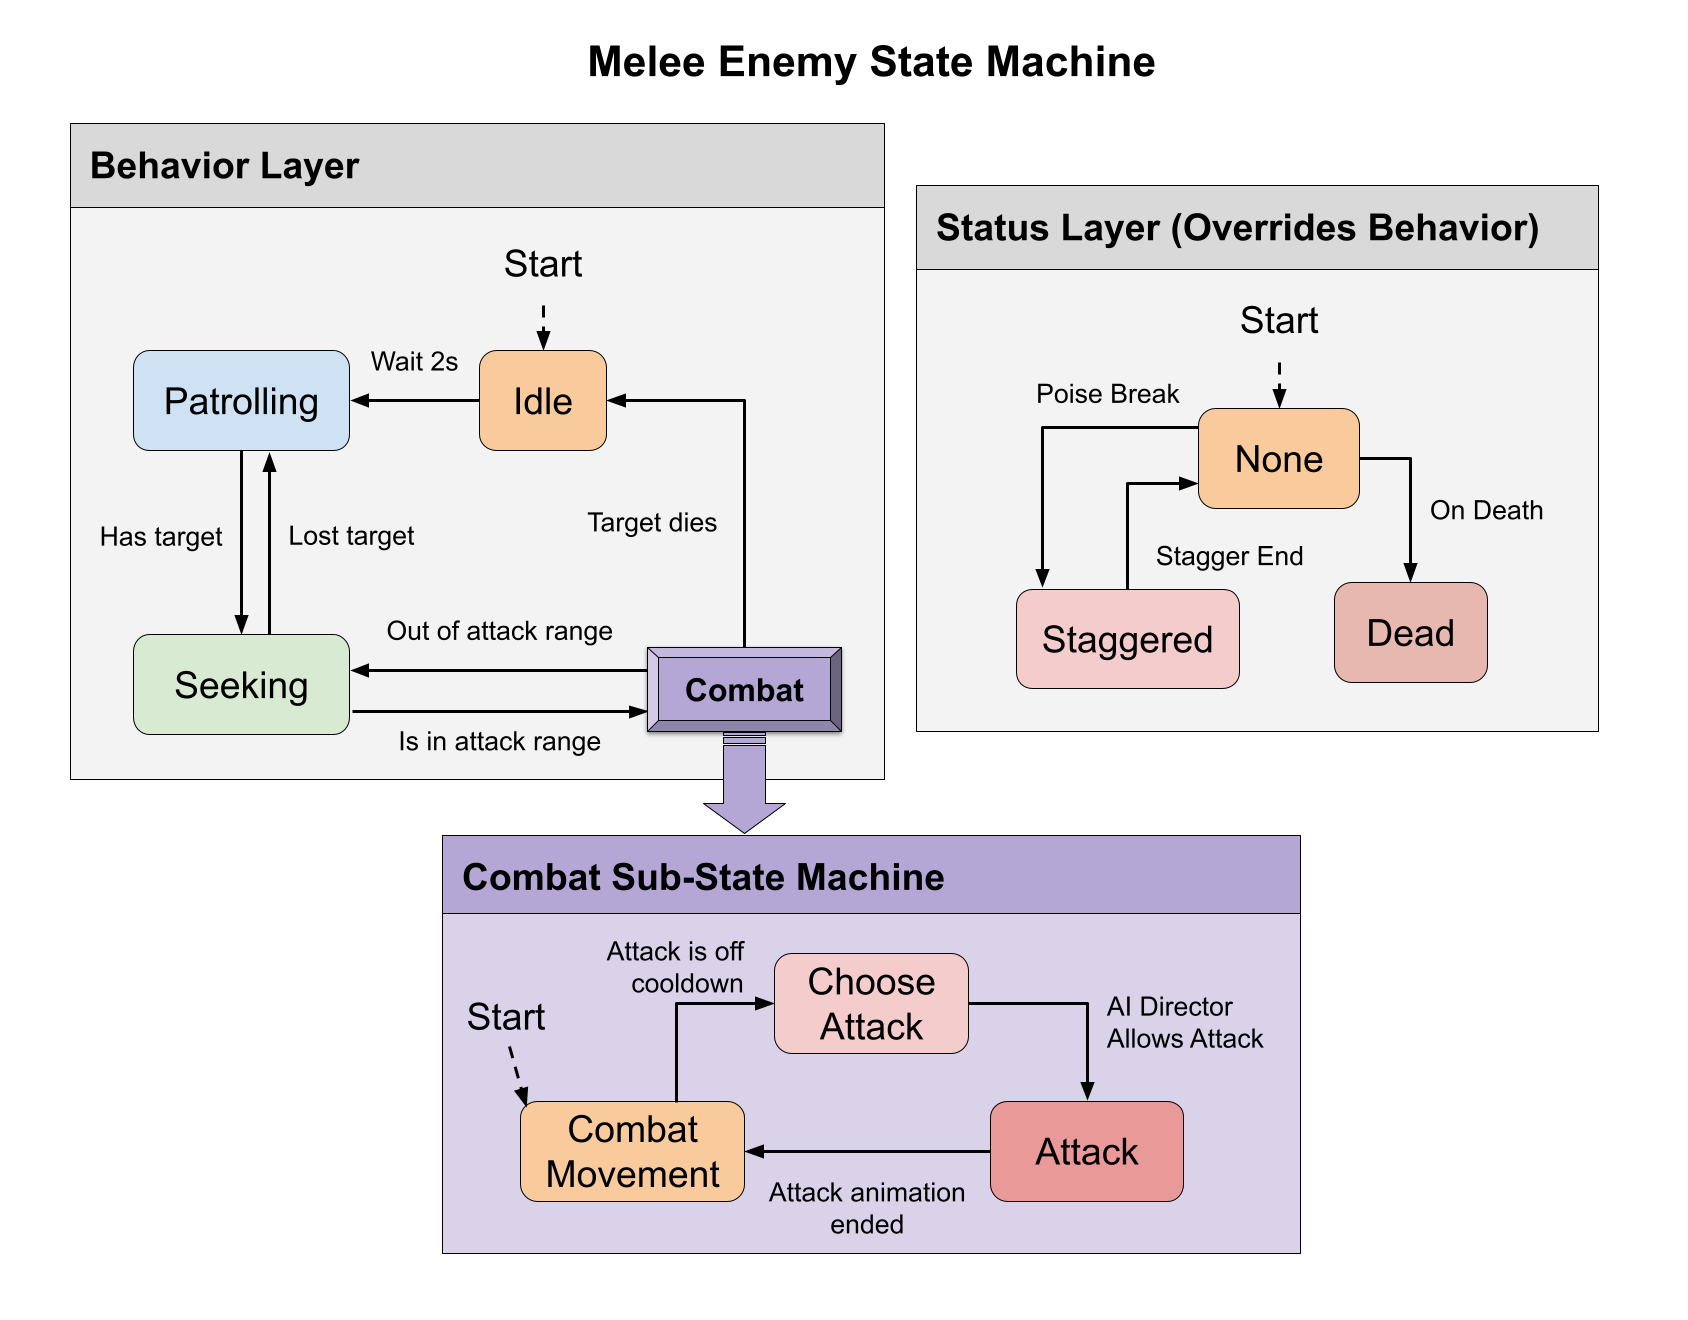
\includegraphics[width=34em]{figures/fig-melee-ai-state-machine.png}
    \end{center}
    \legend{Source: Diagram assembled by authors.}
    \label{fig:fig-ai-state-machine}
\end{figure}

% Implementation of a Serializable, multipurpose State Machine structure
%   - StateMachineController: MonoBehaviours, instanced in scenes. Contains a reference to the state machine and its owner. Validates conditions for transitions, performs transitions and updates states.
We implemented modular and generic State Machines which can be used outside the scope of AI Agents. The reason for this approach was to facilitate the management of player state, helping to constrain the actions which the player can perform given the current game state. We defined a reusable \textsc{StateMachineController} component which can be assigned to a MonoBehaviour. In the context of AI Agents, the StateMachineController is attached to an \textsc{AICharacter}, which represents any AI-controlled agents. The \textsc{StateMachineController} contains a reference to the \textsc{StateMachine} and its owner, and is tasked with performing frame-bound updates to states and validating transition conditions that toggle state changes.

% - State Machines are bound to asset files
% - Class Definitions:States, Transitions, StateBehaviors
%   - StateMachine: Class definition for all the serialized data involving our implementation of state machines. Contains states and transitions. 
%   - States: Contain a variable set of Behaviors, that can be assigned dynamically during runtime and serialization.
%   - Transitions: References an origin and a target state, and contains a set of boolean conditions to validate a transition as valid.
% Each state has a set of dynamically assigned Behaviors that determine the actions performed by an AI Agent on that state.
The definitions of State Machine, including their States, Transitions and Behaviors are constrained to serializable space, being bound to asset files that are referenced by the \textsc{StateMachineController}. The \textsc{StateMachine} class contains serialization data used by \textsc{States}. Each State contains a variable set of \emph{Transitions} and \emph{Behaviors}.

Transitions reference an origin and a target state, and contain a set of boolean validation functions that define when such transition occurs. Behaviors determine the actions can be performed by the State Machine owner. In table \ref{tab:ai-behaviors}, we define all AI Agent behaviors in our implementation, specifying the States in which they are used and a brief description of the actions performed by the AI Agent when executing the Behavior.

% * Table - AICharacter Behaviors
% =================================================================================
% Name           | Related States   | Description
% =================================================================================
% WaypointMove   | Patrolling       | Uses a set of waypoints (which can be empty)
%                |                  | to move a character in fixed points on the
%                |                  | NavMesh of the environment.
% ---------------|------------------|----------------------------------------------
% Scan           | Idle, Patrolling | Uses a set of collision triggers to detect
%                |                  | enemies of the AI agent in an area around or
%                |                  | in front of its position, and assigns a 
%                |                  | target upon detection.
% ---------------|------------------|----------------------------------------------
% Seek           | Seeking          | Follows a target, constantly moving to its
%                |                  | position until the target is out of range.
% ---------------|------------------|----------------------------------------------
% AdjustDistance | CombatMovement   | Adjusts the distance of the AI Agent to be
%                |                  | close enough to perform an attack, without
%                |                  | being too close to the target.
% ---------------|------------------|----------------------------------------------
% PlanAttack     | CombatMovement   | Chooses the next attack based on the actions
%                |                  | being performed by the target, or by using
%                |                  | random number generation.
% ---------------|------------------|----------------------------------------------
% Attack         | CombatMovement   | Performs the chosen attack on the target
%                |                  | using the Attack System pipeline.
% ---------------|------------------|----------------------------------------------
% RotateAttack   | CombatMovement   | Performs body rotation to adjust the attack
%                |                  | to a moving target. The rotation has limited
%                |                  | speed to permit the target to dodge.
% ---------------|------------------|----------------------------------------------
% Shoot          | Shooting         | Used by ranged enemies. Continuously shoot
%                |                  | arrows at a target until the target is
%                |                  | out of range.
% ---------------|------------------|----------------------------------------------
% Death          | Dead             | Deactivates all components, triggers the
%                |                  | death animation and de-spawns the AI agent.
% =================================================================================

\begin{table}[!h]
    \begin{center}
      \caption{A list of the behaviors in the States of the AI Agents in our implementation.}
      \label{tab:ai-behaviors}
      \rowcolors{2}{}{gray!25} % Alternate row colors
      \begin{tabular}{ >{\small}w{l}{6em} >{\small}w{l}{7em} >{\small}m{17em} } % alignments and column size
        \addlinespace
        \toprule
        % Headings
        \bf Name       & \bf Related States  & \bf Description                              \\
        \midrule
        WaypointMove   & Patrolling          & Uses a set of waypoints (which can be empty)
                                               to move a character in fixed points on the 
                                               NavMesh of the environment.                  \\
        Scan           & Idle, Patrolling    & Uses a set of collision triggers to detect   
                                               enemies of the AI agent in an area around
                                               or in front of its position, and assigns a 
                                               target upon detection.                       \\
        Seek           & Seeking             & Follows a target, constantly moving to its
                                               position until the target is out of range.   \\
        AdjustDistance & CombatMovement      & Adjusts the distance of the AI Agent to be 
                                               close enough to perform an attack, without
                                               being too close to the target.               \\
        PlanAttack     & CombatMovement      & Chooses the next attack based on the actions 
                                               being performed by the target, or by using
                                               random number generation.                    \\
        Attack         & CombatMovement      & Performs the chosen attack on the target 
                                               using the Attack System pipeline.            \\
        RotateAttack   & CombatMovement      & Performs body rotation to adjust the attack 
                                               to a moving target. The rotation has limited 
                                               speed to permit the target to dodge.         \\
        Shoot          & Shooting            & Used by ranged enemies. Continuously shoot 
                                               arrows at a target until the target is 
                                               out of range.                                \\
        Death          & Dead                & Deactivates all components, triggers the 
                                               death animation and de-spawns the AI agent.  \\
        \bottomrule
      \end{tabular}
    \end{center}
  \end{table}

% State machines are serialized, therefore Behaviors are unable to keep state of objects that are instanced in a scene. We need to keep data for each behavior in the container of the state machine, which in this case is the AICharacter.
States are serialized and independent of instanced objects, which creates the restriction that Behaviors are unable to store runtime data representing entity state. Therefore, we are required to maintain the data used by each behavior in a container for the \textsc{StateMachineController}. For this reason, we create the \textsc{IStateMachineOwner} interface, which provides a public accessor to a \textsc{Hashmap} structure which contains the runtime and referenced data for an instanced entity, using an identifier for the current state as the \emph{Key}. Figure \ref{fig:state-machine-class-diagram} shows the class and data structure relationships for our implementation of state machines. 

% * Figure: State Machine system architecture
\begin{figure}[!ht]
    \begin{center}
    \caption{Class relationship for our State Machine implementation from the perspective of AI Systems.}
    \vspace{0.5em}
        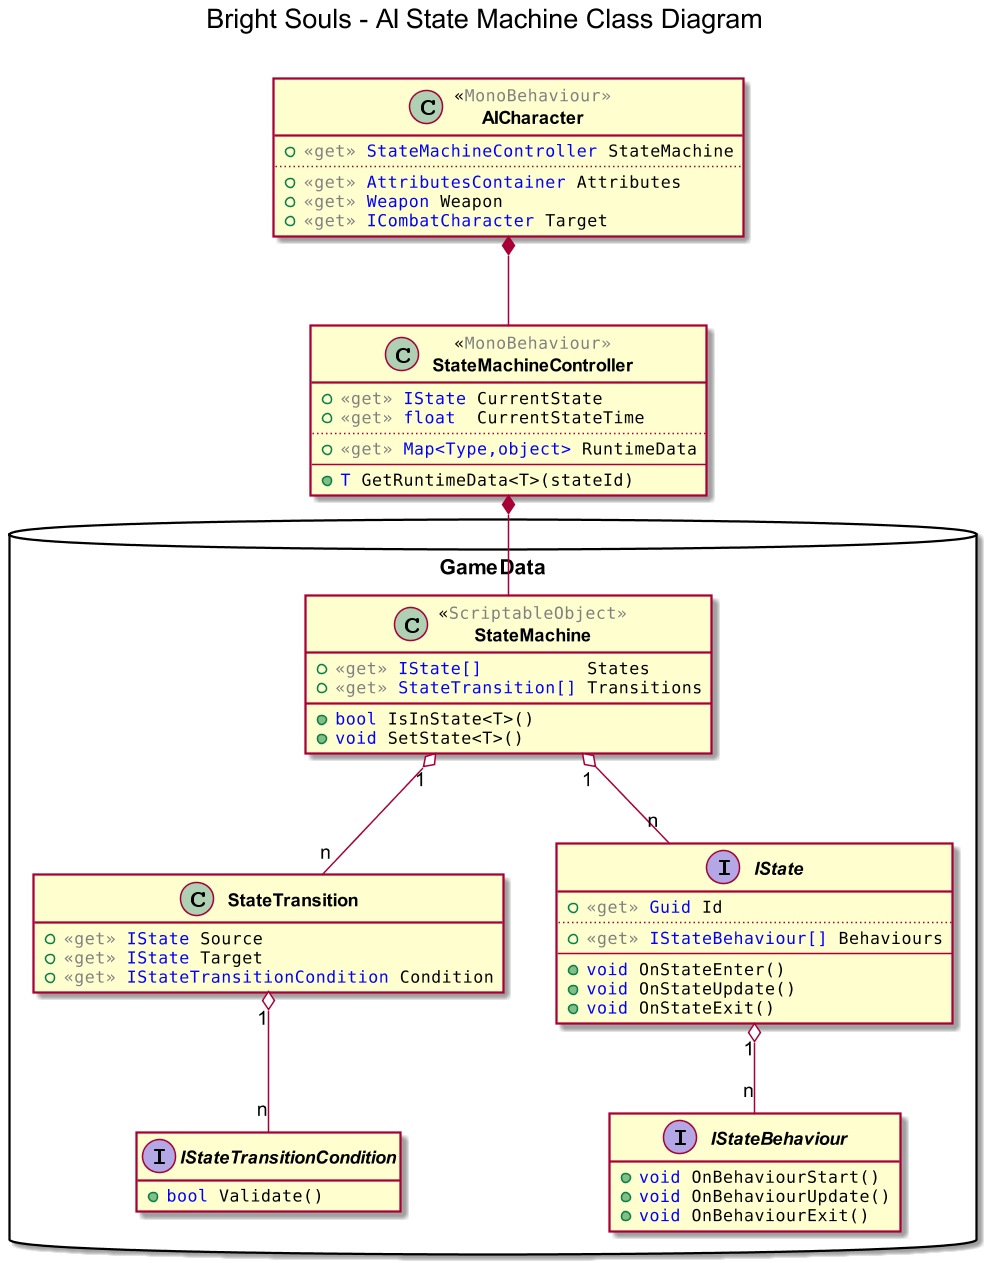
\includegraphics[width=28em]{figures/fig-state-machine-class-diagram.png}
        \legend{Source: Diagram assembled by authors.}
    \end{center}
    \label{fig:state-machine-class-diagram}
\end{figure}

% ===================================================================
% ===================================================================
% ===================================================================

\subsection{Implementation of Behaviors}

\sepfootnotecontent{fn:manhattan-distance}{\emph{Manhattan distance} is a simplified distance estimation between two points in a vector space. It is commonly used in realtime pathfinding algorithms due to its low computational cost.}

% Movement:
%   - Use of NavMeshes to define walkable space in 3D environment for AI Agents.
%   - Use of A* path-finding algorithm to define movement over nodes scattered throughout the mesh.
To implement AI Agent pathfinding when executing the \textsc{WaypointMove} or \textsc{Seek} behaviors, we use Unity's \emph{NavMesh} system, which uses the topology of 3D objects and predefined movement costs to generate a planar mesh representing traversable surfaces. The resulting mesh also contains weights for each vertex, which causes the AI Agent to prioritize certain paths which are considered optimal. Using  data generated from \emph{NavMeshes}, we define the movement path as a set of positions calculated by the \textsc{A*} algorithm, using the \emph{Manhattan Distance}\sepfootnote{fn:manhattan-distance} function as an estimation heuristic.

% How AI agents scan for targets
% - Spheric collider for frontal view cone
%      - Detects collision with ICombatCharacters from different Faction
% - Calculate the angle between agent forward and target relative pos
To scan for targets in the environment and initiate combat, AI Agents contain a spheric collider representing a radius where targets can be detected. We constrain such targets to those within a frontal view cone defined by the agent's orientation.  We validate whether an entity is inside an agent's view cone using the \emph{Target's Relative Direction}, which can be calculated by subtracting the agent's position from the target's position, normalizing the result and projecting it onto the ground plane. We then use Unity's \textsc{Vector3.Angle} operation to compare agent orientation and the target's relative direction, and clamp results to a cone of 90 degrees.

When an entity of the type \textsc{ICombatCharacter} enters the resulting area, such entity is marked as an \emph{Elligible target}. Elligible targets are then further restricted by the value of their \textsc{FactionAttribute}, where a valid target must belong to a different faction to the agent. The agent will then mark the first detected elligible entity as their target, and proceed to chase them.

% - What happens when the target dies
%       - AI agent is reset to Idle
% - If target is unreachable, same thing happens
Therefore, when an enemy AI agent is able to defeat their target, they are reset to the \emph{Idle} state. A similar event happens when the AI agent is in the \emph{Seeking} state and the target can not be reached. If the target is in an unreachable position where there is no traversable ground geometry from the agent to their target, the AI loses interest in the target and returns to its default state.

% How AI Agents attack
%   - Each enemy has own state machine
%   - State state differs because of behaviors and data
%   - CombatMovement: adjust position, plan attack, execute
To differentiate the behaviors of different enemies, we created state machine definitions based on \emph{Enemy Types}. Each enemy type has their own state machine definition, with different behaviors for each state. For melee-ranged agents, we defined the unique \textsc{CombatMovement} state. In such state, AI agents adjust their position and execute attacks based on target state and environment properties. The \textsc{CombatMovement} functions as a sub-state machine, where we switch between three stages to give the impression of different states: \textsc{PositionAdjustment}, \textsc{AttackPlanning} and \textsc{AttackExecution}.

% AdjustPosition
%     - Two-dimensional radial and distance-based positioning
In the \textsc{PositionAdjustment} stage, we perform several steps to calculate the position to which an agent should move towards. First, we define a \emph{distance relationship} between the agent and their target; Then, we define a \emph{radial distribution position}, which constrains the agent to a directional range in a circular perimeter around the target.

\sepfootnotecontent{fn:group-ai-brain}{The \textsc{GroupAIBrain} component is a manager to all AI agents engaged in a \emph{Combat Encounter} against the player.}

\sepfootnotecontent{fn:hitbox-central-point}{The \emph{Hitbox central point} refers to a hypothetic central point between the limits of a bounding box that envelops all \emph{Hitboxes} of a game entity.}

%     - GroupAIBrain: What is the expected distance?
To define the \emph{distance relationship} between the agent and their target, we query the \textsc{GroupAIBrain}\sepfootnote{fn:group-ai-brain} component to check if the player is dealing with too many enemies. In that case, the agent takes an idle stance and remains in the backline, avoiding direct conflict with their target. Similarly, we determine if the AI agent attacks are on \emph{cooldown}, which also positions the agent throughout the backline. We then calculate the average \emph{Hitbox Central Point}\sepfootnote{fn:hitbox-central-point} distance for all attacks that the AI Agent can perform. We use this average to create a target position that maximizes the chances of hitting the target. The agent adjusts their distance towards or away from their target, and executes the attack.

\sepfootnotecontent{fn:combat-encounter}{AI Agents are considered to be in a combat encounter when the player is within their effective combat range. For melee-ranged enemies, this is determined by being in the \textsc{CombatMovement} state.}

% - GroupAIBrain: What is the expected radial position?
%     - Priority index
%     - Positions in arc in circular perimeter
%     - Arc boundaries restricted by environment geometry
%     - Arc also restricted by dynamic radian in GroupAIBrain
To define the radial-distribution position for an entity, the AI Agent is assigned a numeric priority index upon entering the \emph{Combat Encounter}\sepfootnote{fn:combat-encounter}. The value of the priority index is used to evenly arrange AI Agents in an arc of a circular perimeter around the player. The aperture of the arc is defined by environmental geometry around the player and dynamic adjustment metrics. If the arc boundaries are not restricted by environmental geometry, the aperture is defined by an adjustable radian supplied by the \textsc{GroupAIBrain} component.

% - How agents are distributed in the arc
% - Arc divided in equal size segment
% - First agent in center
% - Second and third agent in boundaries
The arc is divided in equal size segments that distribute agents uniformly around the player. At the beginning of a combat encounter, a single agent becomes part of the AI group. This initial agent is defined as the pivot for the group. The arc is divided in two segments centered at the pivot. The following two agents are placed at the outer boundaries of the arc, each at the limits of their respective segments. Every subsequent agent subdivides the largest segment that is closest to the pivot, using the center position of the segment and creating two new segments.

% - Subsequent agents subdivides largest segments from center outwards
% - Recalculate segments when agents die
When the pivot agent is defeated, a new pivot is selected based on its distance from the original pivot, and the segments are recalculated. We iteratively add each subsequent agent which is closest to the pivot through the same algorithm. When non-pivot agents are defeated the group is also recalculated, but we retain the same pivot when recalculating segments. This algorithm is exemplified by figure \ref{fig:arc-segments}, and the resulting behavior is exemplified by figure \ref{fig:enemy-positioning-example}.

% * Figure: Figure illustrating the behavior of the "arc segments" algorithm
\begin{figure}[!ht]
    \caption{Illustration of the "Arc Segments" algorithm for radial positioning of AI Agents around the player character.}
    \begin{center}
        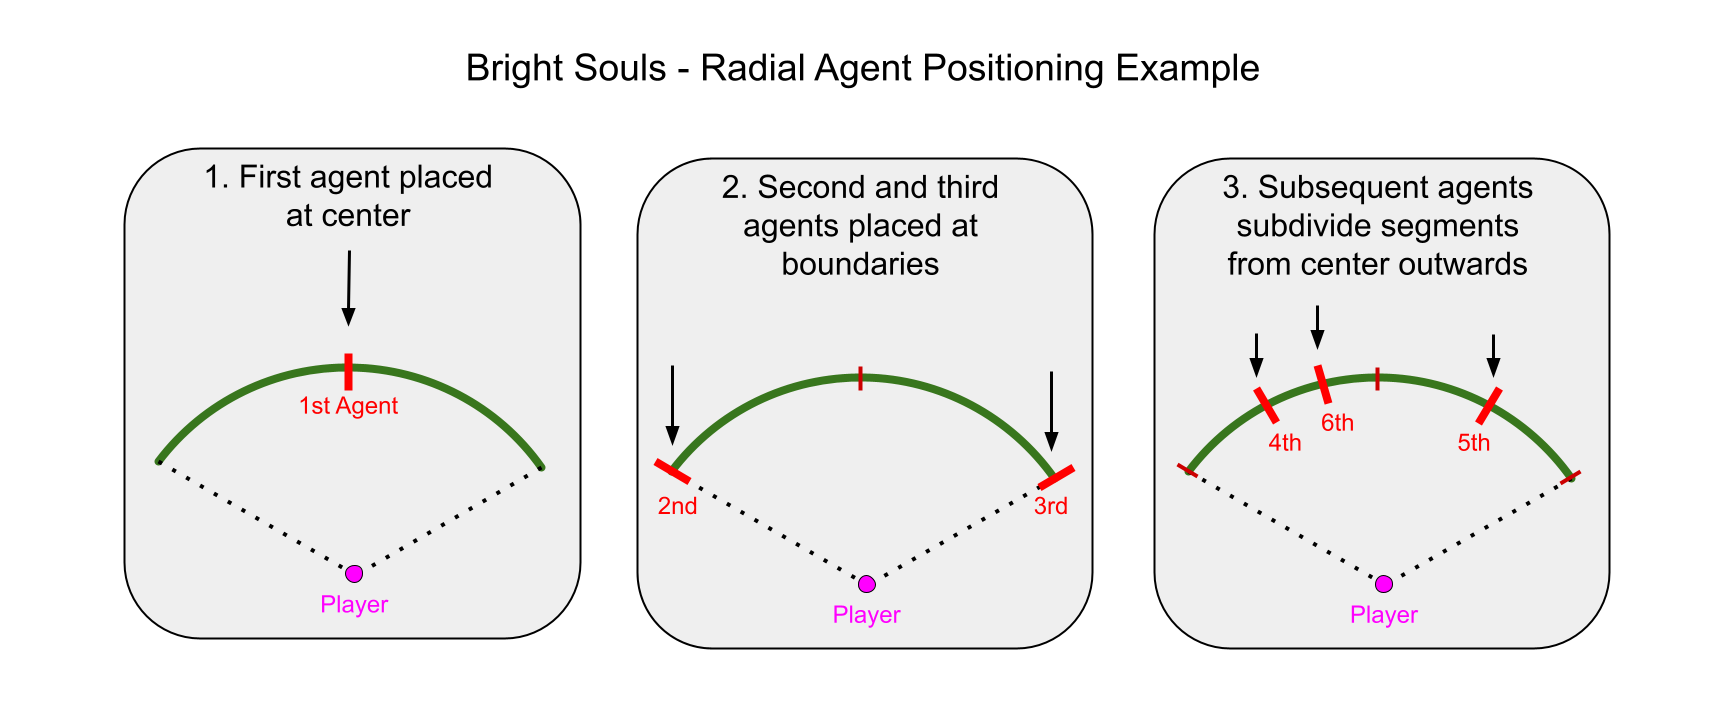
\includegraphics[width=32em]{figures/fig-arc-segments.png}
    \end{center}
    \legend{Source: Diagram assembled by authors.}
    \label{fig:arc-segments}
\end{figure}

% * Figure: Enemy typical radial placement around the player character
\begin{figure}[!ht]
    \caption{An example of melee enemy group positioning with five AI Agent enemies.}
    \begin{center}
        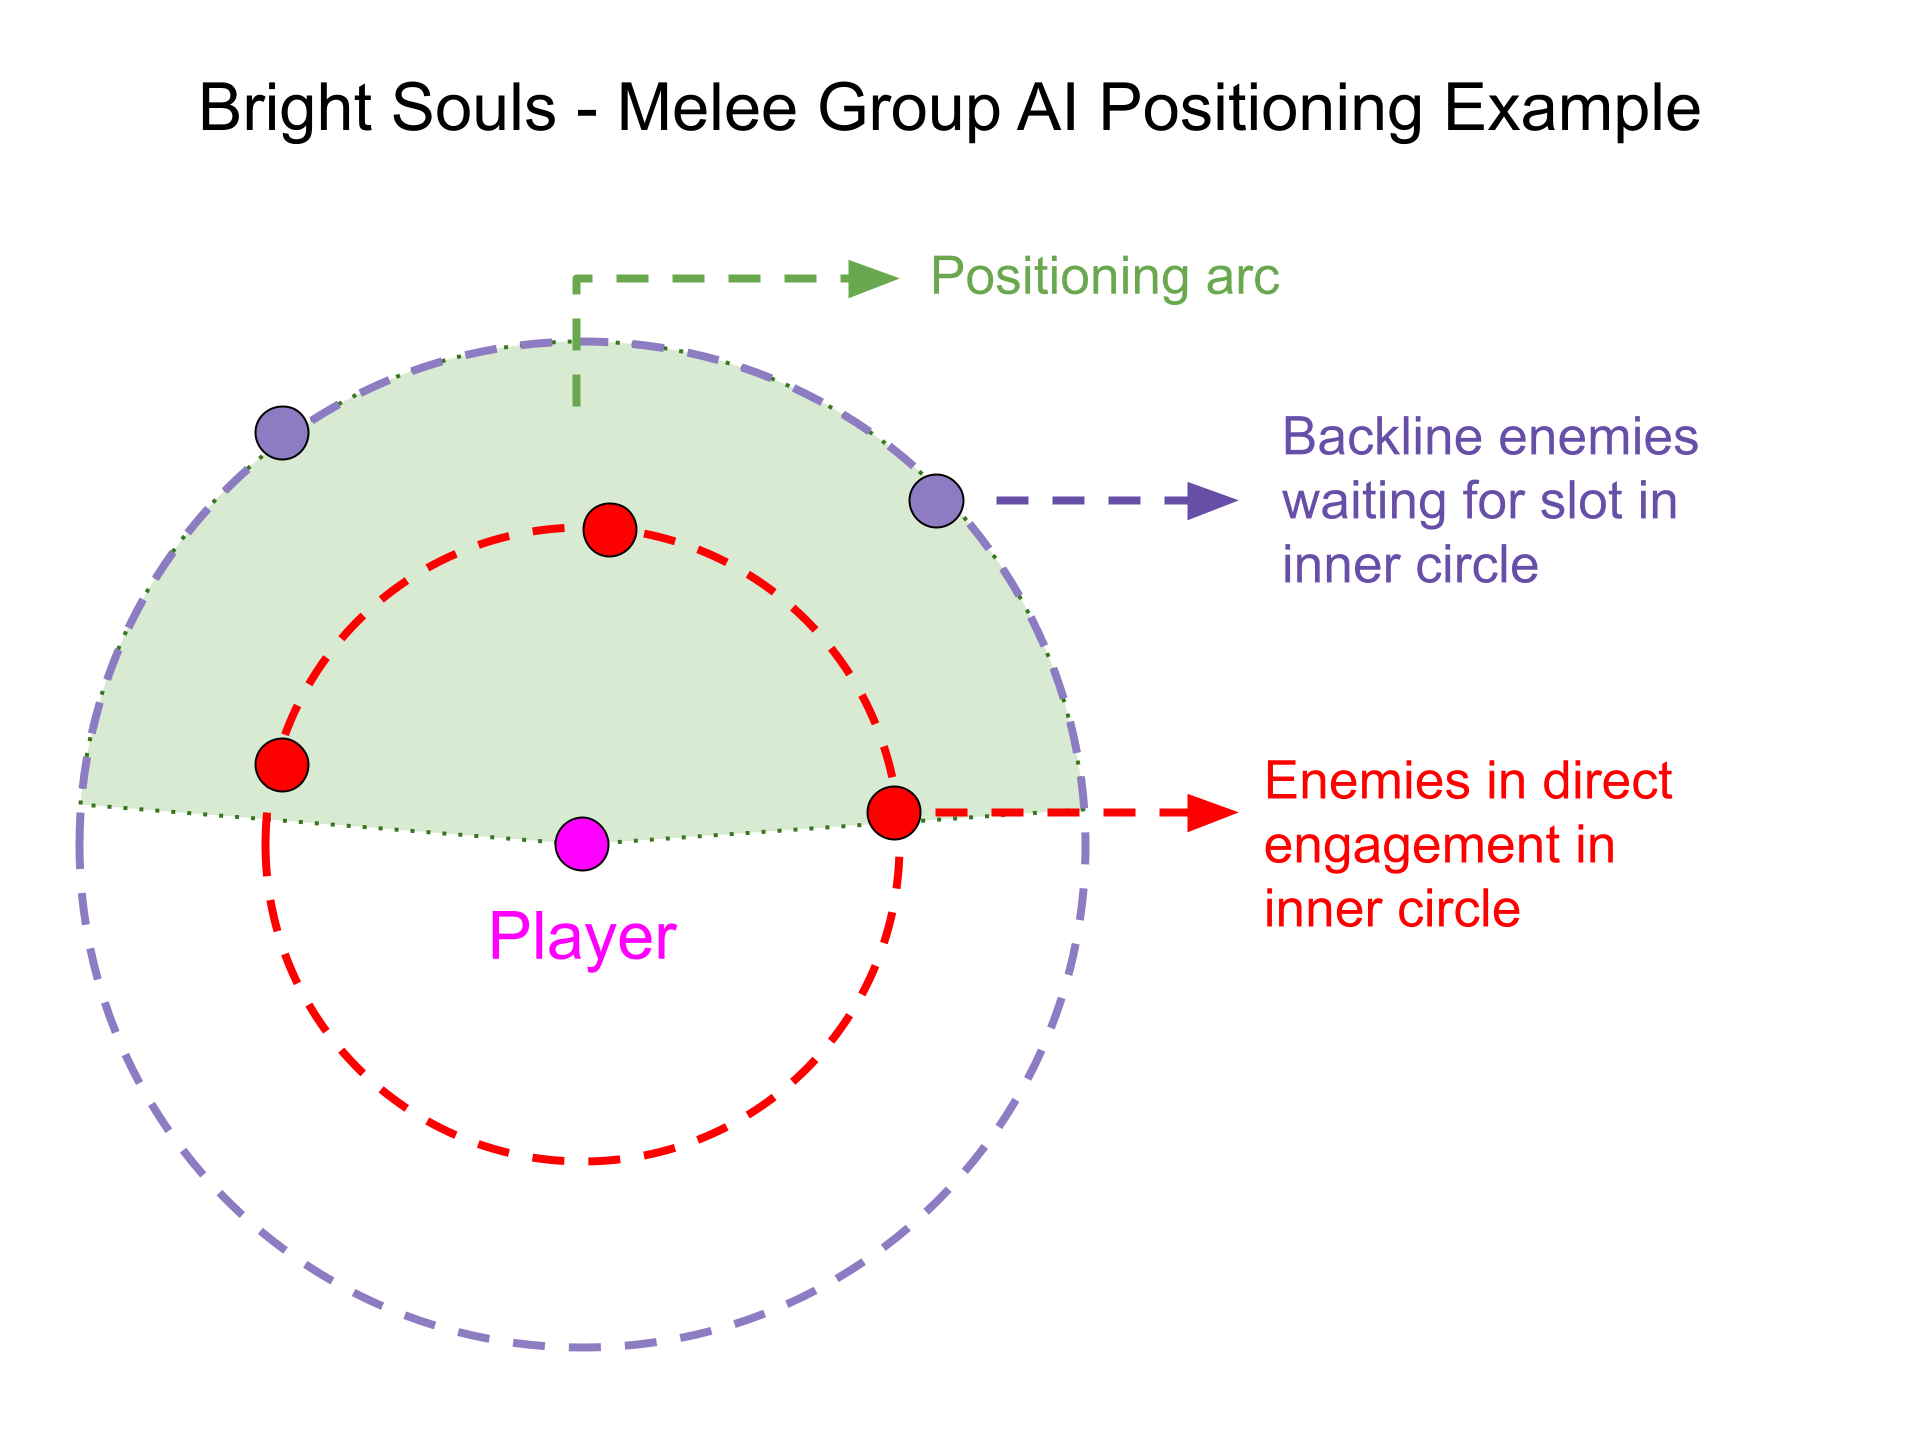
\includegraphics[width=26em]{figures/fig-enemy-positioning-example.png}
    \end{center}
    \legend{Source: Diagram assembled by authors.}
    \label{fig:enemy-positioning-example}
\end{figure}

% PlanAttack behavior
% Player State + GroupAIBrain info used as input
% Decide if can attack and which attack
In the \textsc{PlanAttack} behavior, we use information regarding player state and constraints imposed by the \textsc{GroupAIBrain} component to define if an attack can be executed, and which attack an AI Agent should perform. Each attack has a different purpose designed to guide the player towards a specific response.

%     - AI Brain: Does it give permission to attack?
%     - EGCD: Enemy Group Cool-Down
First, we query the \textsc{GroupAIBrain} component to check whether the agent has permission to attack. Enemy AI Groups have shared  \emph{Enemy Group Cooldown} timers that reset when an agent performs an attack. Agents that are part of a group will be unable to attack unless at least one cooldown timers is available for use. The numbers of timers available and the cooldown time are determined by adaptive parameters from the \textsc{GroupAIBrain} component, and are further discussed in section \ref{sec:adjustments}.

% Uses list of available types to query for information
%     - AI Brain: does it give permission for special attack?
Second, the PlanAttack behavior uses information on attack types available to the entity to query which information is necessary to decide the attack. We communicate with the \textsc{GroupAIBrain} component to determine if the entity is able to perform \emph{Special Attacks}. Given a small interval of time, a limited number of non-basic attacks can be performed by an agent. If the agent is unable to perform a Special Attack after querying availability from the \textsc{GroupAIBrain} component, it simply chooses one of multiple basic attacks to perform.

Special attacks have the purpose of creating incentive for the player to vary their reactions. For instance, the \emph{Overhead} and \emph{Pierce} attacks are designed to punish the player if attempted to be blocked, and drain a significant amount of the Stamina resource. If the player does attempt to block one of such attacks, they will quickly find themselves out of Stamina and trigger a \emph{Poise Break}\sepfootnote{fn:poise-break} status.

%     - Is the player out of attack range?
%     - How often does the player back-step
Then, we check if the player is still out of attack range after adjusting its position during the \emph{PositionAdjustment} behavior. In such case, we use a parametrized threshold as a probability for the agent to perform a \emph{Charge} attack, if it is one the available special movements. The threshold is combined with a metric from our DDA system regarding the frequency of player back-steps, which affects RNG (random number generation) probabilities for the \emph{Charge} attack. The parametrized thresholds for each attack type are explained further in section \ref{sec:adjustments}. If the agent is not able to perform the \emph{Charge} attack, it is reverted back to the \emph{PositionAdjustment} behavior.

%         - Is the player blocking?
%         - How often does the player block, dodge?
Similarly, we check if the player is blocking and use a threshold for  a \emph{Anti-Block} attacks, such as the \emph{Overhead} or \emph{Pierce} attacks. We combine the threshold with the frequency of player Blocks, and use the resulting value as an input probability for the \emph{Anti-Block} attack. Anti-dodge attacks also use the same approach, with the exception that we disregard current player state. Since the dodging action is discrete and occurs in a fraction of a second, the agent attempts to predict when a player would perform a dodge solely through statistical data.

% ===================================================================
% ===================================================================
% ===================================================================

% TODO \subsubsection{Management of Agent Groups}
%\label{sec:ai-brain}

% ===================================================================
% ===================================================================
% ===================================================================

% TODO \subsection{Design of Enemy Types (ADDITIONAL)}

% TODO Table - Enemy Types
%
% =========|============|========|===========|=========|==========================================
%  Name    | Move Speed | Damage | Atk Speed | Health  | Description                             
% =========|============|========|===========|=========|==========================================
% Ghoul    | Slowest    | Lowest | Slow      | Lowest  | Slow and weak enemy. Introductory enemy 
%          |            |        |           |         | for player to test mechanics.
% ---------|------------|--------|-----------|---------|------------------------------------------
% Skeleton | Fast       | Low    | Medium    | Low     | Fast enemy. Causes player to reposition 
%          |            |        |           |         | and protects archers.                  
% ---------|------------|--------|-----------|---------|------------------------------------------
% Warrior  | Slow       | Medium | Slowest   | High    | Uses shield. Hard to kill. Buys time for  
%          |            |        |           |         | all other enemies.  
% ---------|------------|--------|-----------|---------|------------------------------------------ 
% Archer   | Stationary | Low    | Slowest   | Medium  | Meant to slowly drain player health from
%          |            |        |           |         | a distance if not prioritized.           
% ---------|------------|--------|-----------|---------|------------------------------------------
% Knight   | Medium     | High   | Fast      | Highest | Meant to force player to dodge, blocking 
%          |            |        |           |         | his Attacks Drain too much Stamina.      
% =========|============|========|===========|=========|==========================================

% TODO Table - Attack Speed Values (tab:attack-speed-values)
%
% ==========|======|===========
% Atk Speed | APS  | Entities
% ==========|======|===========
% Slowest   | 0.33 | Archers,
%           |      | Warriors
% ----------|------|-----------
% Slow      |  0.5 | Ghouls
% ----------|------|-----------
% Medium    |  0.8 | Skeletons
% ----------|------|-----------
% Fast      |  1.5 | Knights
% ----------|------|-----------
% Fastest   |  2.3 | Player
% ==========|======|===========

% TODO Table - Health Values (tab:enemy-health-values)
%
% ========|======|===========
% Health  | PATK | Entities
% ========|======|===========
% Lowest  |    2 | Ghouls
% --------|------|-----------
% Low     |    3 | Skeletons
% --------|------|-----------
% Medium  |    6 | Archers
% --------|------|-----------
% High    |    8 | Warriors
% --------|------|-----------
% Highest |   10 | Knights
% ========|======|===========

% TODO Table - Damage Values (tab:enemy-damage-values)
%
% =======|======|===========
% Damage | ATKP | Entities
% =======|======|===========
% Lowest |   20 | Ghouls
% -------|------|-----------
% Low    |   14 | Archers, 
%        |      | Skeletons
% -------|------|-----------
% Medium |   12 | Warriors
% -------|------|-----------
% High   |    9 | Knights
% =======|======|===========

% TODO Table - Attack Types (tab:enemy-attack-types)
%
% =========|============|==========|===============================
% Name     | Type       | Enemies  | Description
% =========|============|==========|===============================
% Slash    | Basic      | Ghoul,   | Low damage attack, no health
%          |            | Skeleton | damage when blocked. Low poise
%          |            |          | damage.
% ---------|------------|----------|-------------------------------
% Arrow    | Basic      | Archer   | Low damage attack, no damage
%          |            |          | when blocked.
% ---------|------------|----------|-------------------------------
% Double   | Basic      | Knight   | Medium damage attacks, low 
% Slash    |            |          | damage when blocked.
% ---------|------------|----------|-------------------------------
% Charge   | Gap Closer | Skeleton,| Medium damage attack. Enemy
%          |            | Knight   | runs to player to land the
%          |            |          | attack from a long distance.
% ---------|------------|----------|-------------------------------
% Overhead | Anti-Block | Warrior  | Medium damage attack. Consumes
%          |            |          | half of player stamina if
%          |            |          | attempted to be blocked.
% ---------|------------|----------|-------------------------------
% Pierce   | Anti-Block | Knight   | High damage attack. Pierces
%          |            |          | through player defense, 
%          |            |          | consuming most of player
%          |            |          | stamina if blocked.
% ---------|------------|----------|-------------------------------
% Sweep    | Anti-Dodge | Knight   | Medium damage attack. Has
%          |            |          | three hit detection phases
%          |            |          | and a long duration. Meant
%          |            |          | to catch the player in the
%          |            |          | final position after a dodge.
% =========|============|==========|===============================

% ===================================================================
% ===================================================================
% ===================================================================

% TODO \subsection{Level Design (ADDITIONAL)}

% ===================================================================
% ===================================================================
% ===================================================================

\section{Dynamic Adjustments System}

To implement a DDA system which modifies game difficulty to be in harmony with player skill, we need to capture gameplay data which can be translated into skill evaluation metrics. We satisfy this requirement by recording gameplay events in a tabular format, which can be reconstructed after completion of game levels to generate metrics. We calculate such metrics to represent the frequency and efficiency of actions performed by the player during a level. Then, we use such metrics as an input to a comparison with predefined thresholds, which serve as discrete delimiters to predefined parametrized adjustments to difficulty. Figure \ref{fig:adjustments-execution-flow} provides an overview of our implementation of a DDA system, showing the execution flow and interactions between the defined components.

\begin{figure}[!ht]
    \begin{center}
    \caption{Diagram illustrating the execution flow of the dynamic adjustments system in our application.}
        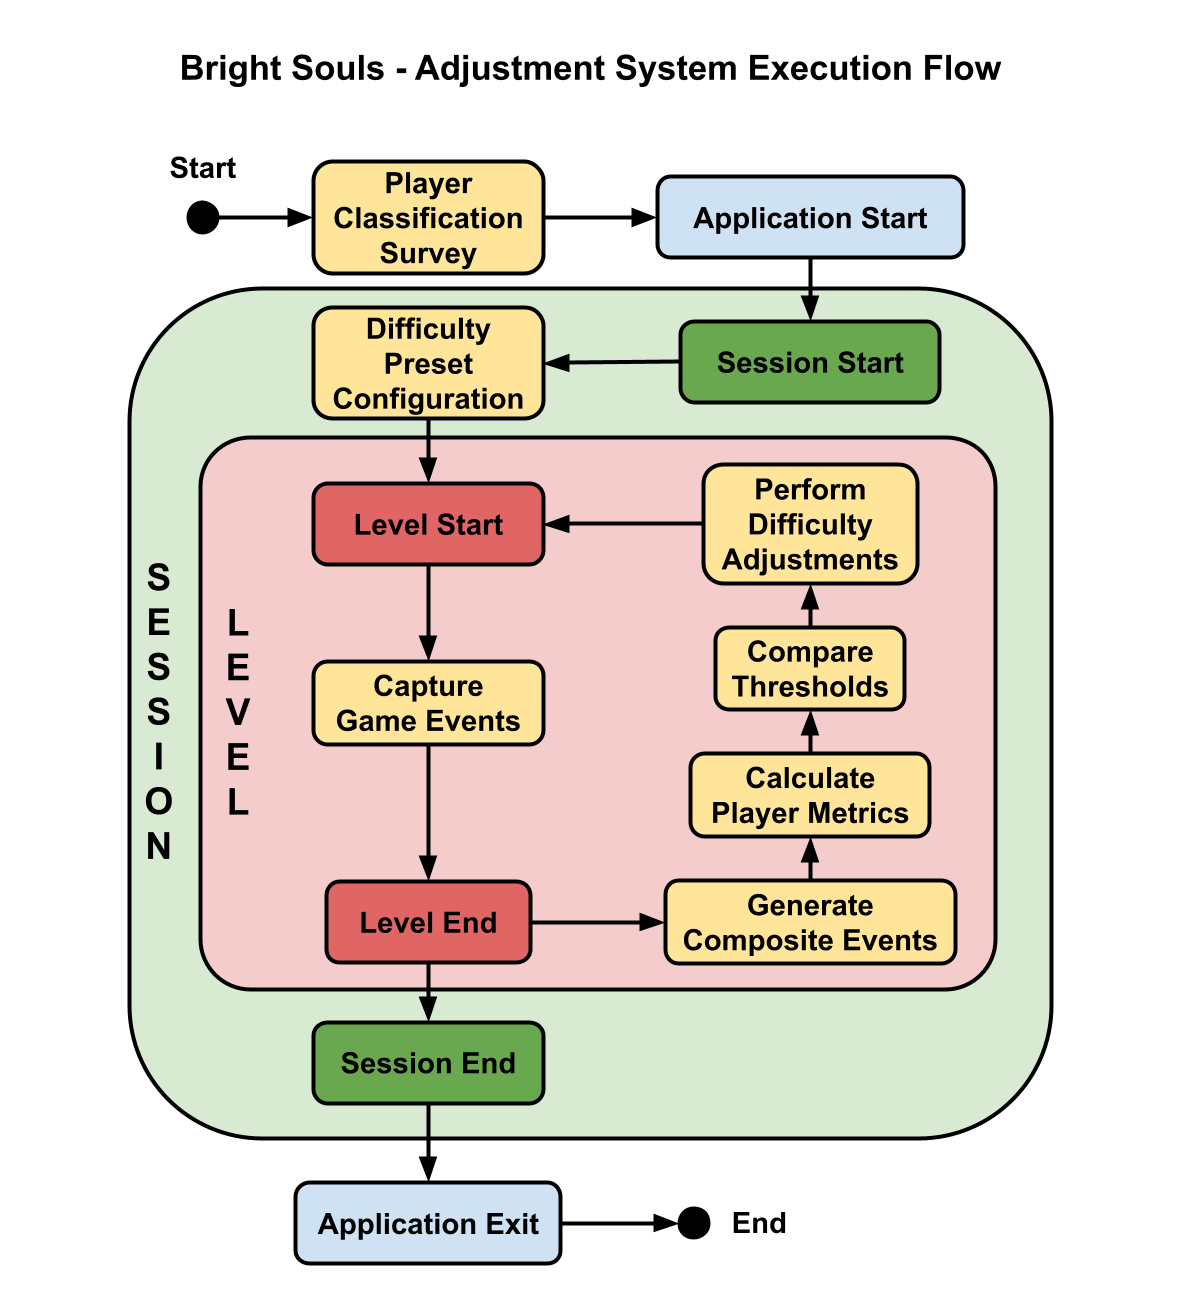
\includegraphics[width=34em]{figures/fig-adjustments-execution-flow.png}
        \legend{Source: Diagram assembled by authors.}
        \label{fig:adjustments-execution-flow}
    \end{center}
\end{figure}

\subsection{Event Tracking Objectives}

We begin the pipeline of our adjustments system through data acquisition, by logging gameplay-related \emph{Events} which are raised during a game level. To do this, we implement a set of components that observe the actions performed by in-game entities and define parametrized events that can gather variable elements of contextual data as input.

Events are packaged into a standardized data structure called \textsc{EventInstance}, where we store: 
\begin{itemize}
    \item{A \emph{Timestamp}, which represents the time since application start where an event was raised;}
    \item{A \emph{Name}, which is used as an identifier and brief descriptor for the contents of the event;}
    \item{A \emph{Type}, which is used to determine the superset of systems where the event is raised;}
    \item{A \emph{Source}, which is used to determine which in-game entity the event is related to;}
    \item{And a set of variable \emph{Parameters} which are valued types that contain relevant contextual data for the event.}
\end{itemize}

Table \ref{tab:event-instance} shows a description of the fields in the \textsc{EventInstance} data structure, along with the associated types for each field.

% * Table: Event Instances
% Event Instance
%   • Timestamp ( Time : double )
%   • Name ( String )
%   • Type ( String )
%   • Source ( ObjectId : GUID )
%   • Params[]
%       • { "name", "type", "value" }

\begin{table}
    \begin{center}
      \caption{A description of the fields associated with an \textsc{EventInstance}.}
      \label{tab:event-instance}
      \rowcolors{2}{}{gray!25} % Alternate row colors
      \begin{tabular}{ >{\small}w{l}{5em} m{7em} m{16em} } % alignments and column size
        \addlinespace
        \toprule
        % Headings
        \bf Field Name & \bf Field Type  & \bf Description \\
        \midrule
        % Data
        Timestamp      & double          & The time since application start when an event was 
                                           raised. Measured in seconds.                        \\
        Name           & String          & The Name Identifier for an event.                   \\
        Type           & String          & The System from which the event is raised from.     \\
        Source         & ObjectId        & The source in-game entity which caused the event to 
                                           be raised.                                          \\
        Params         & Array of Tuples & A set of data parameters, given in string format,  
                                           that are used to represent any contextual related 
                                           with the event.                                     \\
        \bottomrule
      \end{tabular}
    \end{center}
\end{table}

% - Write events to file in batches for performance
Events are written to a circular buffer and outputted to a file in batches to minimize performance costs over extended gameplay sessions. By doing this, frame rendering "hiccups" are minimized to few particular moments where events exceed a specific threshold of allocated memory for batches. In most instances throughout our tests, such issues did not occur over the duration of a singular game level. We restrict our use of the IO (Input/Output) system and the processing of gameplay data to level transitions. Since players do not have control over the application during loading screens, this solution abstracts data processing from the player, maintaining a fluid gameplay experience.

\sepfootnotecontent{fn:play-session}{A Play Session is delimited by the moment where a user starts the game application and the moment where the user exits the application, returning to the operating system.}

% - Events are stored in a simple .csv file
% - .csv file is uploaded to google sheets after session
For each \emph{Play Session}\sepfootnote{fn:play-session}, we store a unique \emph{CSV} (Comma-Separated Values) file that serves as a simplified database to store in-game events. Before the end of a play session and after all levels are completed by the player, our database files are uploaded to a \emph{Google Sheets} folder using the \emph{Sheets API}.

\subsection{Captured Events}

In our implementation, we differentiate between \emph{discrete} events and \emph{timer-based} events, which are both part of the \emph{basic events} category; and the aggregation of such instances into \emph{composite} events. Such division is used to facilitate the algorithm for calculating specific player metrics, and to provide a layer of abstraction for users of the event tracking API.

% ========================================
%  Base Events
% ========================================

% Event types
%   - Raised, Timer-based, Composite
Discrete events can be raised at any given moment in a session, and originate from signals emitted by entity components. An example of a discrete event would be the player character performing an attack, where the occurrence of the event depends entirely on input provided by the player and can not be bound to any specific timed measure. Discrete events are used to represent system-based state changes, entity actions and the results of such actions. In table \ref{tab:discrete-events}, we specify the discrete events defined in our implementation.

% * Table - Discrete Events
% TODO Table - Discrete Events
%
%   Game Loop
%       • Session Started
%           • { "sessionId" , GUID  }
%       • Session Ended
%           • { "sessionId" , GUID  }
%       • Level Started
%           • { "levelNumber" , int  }
%           • { "levelLayout" , GUID }
%       • Level Ended
%           • { "levelNumber" , int  }
%           • { "levelLayout" , GUID }
%   Encounter
%       • Encounter Started
%           • { "encounterId" , GUID  }
%       • Encounter Ended
%           • { "encounterId" , GUID  }
%       • Entity Entered Encounter
%           • { "encounterId" , GUID  }
%   Action
%       • Attack Start
%           • { "attackId" , "GUID" }
%       • Attack End
%           • { "attackId" , "GUID" }
%       • Block Start
%       • Block End
%       • Dodge Start
%           • { "position"  , "Vector3" }
%           • { "direction" , "Vector3" }
%       • Dodge End
%           • { "position"  , "Vector3" }
%   Response
%       • Hit Entity
%           • { "target" , "GUID"  }
%           • { "damage" , "float" }
%       • Hit by Entity 
%           • { "attacker" , "GUID"  }
%           • { "damage"   , "float" }
%       • Blocked Attack
%       • Dodged Attack
%       • Staggered
%       • Death

\begin{table}
    \begin{center}
      \caption{A list of the discrete events captured over a play session in our implementation.}
      \label{tab:discrete-events}
      \rowcolors{2}{}{gray!25} % Alternate row colors
      \begin{tabular}{ w{l}{7em} m{6em} w{l}{9em} m{10em} } % alignments and column size
        \addlinespace
        \toprule
        % Headings
        \bf Name & \bf Category & \bf Parameters & \bf Description \\
        \midrule
        % Game System Events
        Session Start & GameSystem & sessionId : GUID & User started and loaded the application. \\
        Session End   & GameSystem & sessionId : GUID & User quit the application. \\
        Level Start   & GameSystem & \makecell[l]{levelNumber : int\\levelLayout : GUID} & Player started a level. \\
        Level End     & GameSystem & \makecell[l]{levelNumber : int\\levelLayout : GUID} & Player finished level. \\
        \midrule
        % Encounter Events
        Encounter Start & Encounter & encounterId : GUID & User started and loaded the application. \\
        Encounter End   & Encounter & encounterId : GUID & User started and loaded the application. \\
        \makecell[l]{Entity Enter\\Encounter} & Encounter & encounterId : GUID & User started and loaded the application. \\
        \midrule
        % Action Events
        \midrule
        % Response Events
        \bottomrule
      \end{tabular}
    \end{center}
\end{table}

In contrast, timer-based events are raised repeatedly at fixed time intervals over the course of a level. They are used to track values and actions that change over the course of time, such as the position of an entity, the movement performed by the player and the proximity of the player to walls and obstacles. Timer-based events use a \emph{polling} approach to determine the value of its parameters, instead of the signal-based system used by discrete events. In table \ref{tab:timer-based-events}, we specify the timer-based events used in our implementation.

% * Table - Timer-Based Events
%
%   • Entity Position
%       • Global Position (Vector3)
%   • Entity Movement
%       • Distance (float)
%       • Direction (Vector3)

\begin{table}[!ht]
    \begin{center}
      \caption{A list of the timer-based events captured in our implementation.}
      \label{tab:timer-based-events}
      \rowcolors{2}{}{gray!25} % Alternate row colors
      \begin{tabular}{ >{\small}w{l}{4em} >{\small}w{c}{3em} >{\small}w{c}{4.5em} >{\small}w{c}{2.5em} >{\small}m{15em} } % alignments and column size
        \addlinespace
        \toprule
        % Headings
        \bf Name & \bf Category & \bf Params & \bf Types & \bf Description \\
        \midrule
        % Entity Events
        Position & Entity & position & Vector3 & The position of an entity at a given time. \\
        \midrule
        Movement & Player & \makecell[c]{distance\\direction} & \makecell[c]{float\\Vector3} & The movement performed by the player in a small time frame. \\
        Health   & Player & value & float & The Health of the Player at a given time. \\
        Stamina  & Player & value & float & The Stamina of the Player at a given time. \\
        \makecell[l]{Available\\Dodge Area} & Player & value & float & The percentage of the area where the player is able to dodge that is not occupied by walls or other obstacles. \\
        \bottomrule
      \end{tabular}
    \end{center}
\end{table}

% Composite Events
%   - Use of composite events as helpers
%   - Composite events are runtime only
Lastly, we define \emph{composite} events by aggregating discrete and timer-based events into a single consolidated package. Composite events are used to simplify the algorithm to calculate specific player metrics. Composite events are not raised or stored during play sessions. Instead, Composite events are generated at runtime between game levels before metric calculation and dynamic adjustments occur.

The aggregation of basic events into composite events uses the \emph{Timestamp}, \emph{Source} and \emph{Parameters} fields to establish the correlation between basic events. We use such fields to guarantee that events of different scopes are not being used to calculate the same metric. For instance, the \emph{Successful Block} event uses the parameter \emph{AttackId} from \emph{AttackStart} events to check if the attack being blocked is the same attack that initiated before or after the player started blocking. Table \ref{tab:composite-events} specifies the composite events used in our implementation. 

% * Table - Composite Events
% * Table - Composite events

\begin{table}[!ht]
    \begin{center}
      \caption{A list of the composite events that are created by aggregating basic events.}
      \label{tab:composite-events}
      \rowcolors{2}{}{gray!25} % Alternate row colors
      \begin{tabular}{ >{\small}w{l}{4em} >{\small}w{c}{4em} >{\small}w{c}{10em} >{\small}m{12em} } % alignments and column size
        \addlinespace
        \toprule
        % Headings
        \bf Name & \bf Category & \bf Base Events & \bf Description \\
        \midrule
        % Session Composite Events
        \makecell[l]{Encounter\\Completed} & Game & \makecell[c]{EncounterStart\\EncounterEnd} & Player successfully eliminated all enemies in an encounter. \\
        \makecell[l]{Level\\Completed} & Game & \makecell[c]{LevelStart\\LevelEnd} & Player successfully completed a level. \\
        \makecell[l]{Session\\Completed} & Game & \makecell[c]{SessionStart\\SessionEnd} & Player finished a play session. \\
        \midrule
        % Combat Composite Events
        \makecell[l]{Successful\\Dodge} & Combat & \makecell[c]{AttackStart,DodgeStart\\!HitByEntity,AttackEnd} & Player successfully dodged an attack. \\

        \makecell[l]{Failed\\Dodge} & Combat & \makecell[c]{AttackStart,DodgeStart\\HitByEntity,AttackEnd} & Player failed to dodge an attack. \\

        \makecell[l]{Successful\\Block} & Combat & \makecell[c]{AttackStart,BlockStart\\BlockedAttack,AttackEnd} & Player successfully blocked an attack. \\

        \makecell[l]{Failed\\Block} & Combat & \makecell[c]{AttackStart,BlockStart\\HitByEntity,DefenseBreak\\AttackEnd} & Player failed to block an attack. \\

        \makecell[l]{Successful\\Avoid} & Combat & \makecell[c]{AttackStart,!HitByAttack\\!BlockStart,!DodgeStart\\AttackEnd} & Player successfully avoided an attack without performing a Dodge or Block. \\

        \makecell[l]{Failed\\Avoid} & Combat & \makecell[c]{AttackStart,HitByAttack\\!BlockStart,!DodgeStart\\AttackEnd} & Player got hit by an attack without performing a Dodge or Block. \\

        \makecell[l]{Offensive\\Action} & Combat & \makecell[c]{AttackStart} & Player performed an offensive action. \\

        \makecell[l]{Defensive\\Action} & Combat & \makecell[c]{DodgeStart,BlockStart\\SuccessfulAvoid} & Player performed a defensive action. \\

        \midrule
        % Entity Composite Events
        \makecell[l]{Entity\\Eliminated} & Entity & \makecell[c]{EncounterStart\\EntityJoinEncounter\\EntityDeath} & Player eliminates an entity after it joins an encounter \\
        \bottomrule
      \end{tabular}
    \end{center}
\end{table}

% TODO Table - Composite Events

%   • Successful Dodge
%       • Attack Start (Enemy)
%       • Dodge Start (Player)
%       • NOT HitByAttack (Player)
%       • Attack End (Enemy)
%   • Failed Dodge
%       • Attack Start (Enemy)
%       • Dodge Start (Player)
%       • Hit By Entity
%       • Attack End (Enemy)
%   • Successful Block
%       • Attack Start (Enemy)
%       • Block Start (Player)
%       • Blocked Attack (Player)
%       • Attack End (Enemy)
%   • Failed Block
%       • Attack Start (Enemy)
%       • Block Start (Player)
%       • Hit By Entity OR Defense Break
%       • Attack End (Enemy)
%   • Successful Avoid
%       • Attack Start (Enemy)
%       • NOT Hit By Attack (Player)
%       • Attack End (Enemy)
%   • Failed Avoid
%       • Attack Start (Enemy)
%       • NOT Block Start (Player)
%       • NOT Dodge Start (Player)
%       • Attack End (Enemy)

\subsection{Player Metrics}

After the player successfully completes a level and we perform aggregation of basic events into composite events, we calculate the metrics which are used as input to perform difficulty adjustments. Reading and performing data transformations over events in our application requires a high processing and \emph{Input/Output} load. Therefore, we chose to postpone calculation of player metrics to  non-interactive segments of our application. This imposes a limitation to our application where we are unable to perform difficulty adjustments in real time. Instead, adjustments are performed on a per-level basis, with metrics being calculated before each level is started.

During our analysis of the object of study, we defined adjustment targets that could affect the player's experience and learning curve. We use such adjustments as a basis to define which metrics are required to be gathered. Metrics are meant to evaluate the efficiency and tendencies of a player. Each difficulty adjustment relates to one or several aspects of the player's skill. Thus, metrics are used to provide an estimation of the efficiency of player decisions or their ability to execute the appropriate actions for each situation.

We categorize metrics into \emph{profile} and \emph{performance} metrics. Profile metrics identify player habits and common responses to the environment or combat encounters. In contrast to metrics discussed in \citet{ARTICLE_DynamicPlayerModelling}, the profile metrics in our implementation are used to create interesting interactions between the player, enemies and the environment. We increase the variety of enemy actions and behaviors based on player success, and adapt level layout complexity depending on the player's use of environment geometry.

We use profile metrics to detect the frequency of defensive actions and target prioritization tendencies. Information regarding player actions is used to modify the chance of enemies performing specific actions, as well as changing their placement in levels.  Table \ref{tab:profile-metrics} provides a list of the profile metrics implemented in our application, along with the events that are used to calculate each metric with a brief description of its purpose.

% * Table - Profile Metrics
% * Table - Profile Metrics

\begin{table}[!ht]
    \begin{center}
      \caption{A list of the \emph{profile metrics} implemented to monitor player habits and common responses to combat situations in our application.}
      \label{tab:profile-metrics}
      \rowcolors{2}{}{gray!25} % Alternate row colors
      \begin{tabular}{ >{\small}w{l}{4.5em} >{\small}w{c}{7em} >{\small}m{16.5em} } % alignments and column size
        \addlinespace
        \toprule
        % Headings
        \bf Name & \bf Related Events & \bf Description \\
        \midrule

        \makecell[l]{Block\\Frequency} & \makecell[c]{SuccessfulBlock\\FailedBlock\\DefensiveAction} & The frequency [0,1] in which the player performs the Block action in comparison to other defensive methods. \\

        \makecell[l]{Dodge\\Frequency} & \makecell[c]{SuccessfulDodge\\FailedDodge\\DefensiveAction} & The frequency [0,1] in which the player performs the Dodge action in comparison to other defensive methods. \\

        \makecell[l]{Avoid\\Frequency} & \makecell[c]{SuccessfulAvoid\\DefensiveAction} & The frequency [0,1] in which the player avoids an attack without blocking or dodging in comparison to other defensive methods. \\

        \makecell[l]{Avg. Enemy\\Lifetime} & \makecell[c]{EncounterStart\\EntityJoinEncounter\\EntityDeath} & The average time it takes for an enemy to die from the moment it joins an encounter. This metric has one instance per enemy type. \\

        \bottomrule
      \end{tabular}
    \end{center}
\end{table}

% Profile

%   Defensive action frequency
%       • Blocking frequency
%       • Dodge frequency
%       • Avoid frequency

%   • Enemy Lifetime
%       - Per enemy lifetime
%       - Scoped in {Encounter, Level, Session}

% Performance Metrics

In contrast, performance metrics focus on the results of player actions. We measure success, failure and the efficiency of execution of game mechanics or strategies. We attempt to use performance metrics to smooth out the learning curve for beginner players, easing the learning process of basic game mechanics. Some examples of adjustments based on performance metrics include the number of enemies that can simultaneously attack the player, visual cues for enemy attacks, the frequency of checkpoints in levels and the overall game speed. Table \ref{tab:performance-metrics} provides a list of the performance metrics implemented in our application, specifying the events used to calculate them and a brief description of their purpose.

% * Table - Performance Metrics
\begin{table}[!ht]
    \begin{center}
      \caption{A list of the \emph{performance metrics} implemented to perform adjustments related to the efficiency and results of player actions.}
      \label{tab:performance-metrics}
      \rowcolors{2}{}{gray!25} % Alternate row colors
      \begin{tabular}{ >{\small}w{l}{4.5em} >{\small}w{c}{7em} >{\small}m{16.5em} } % alignments and column size
        \addlinespace
        \toprule
        % Headings
        \bf Name & \bf Related Events & \bf Description \\
        \midrule

        \makecell[l]{Level\\Duration} & \makecell[c]{LevelStart\\LevelEnd} & The time it takes for the player to clear a level. \\

        \makecell[l]{Encounter\\Duration} & \makecell[c]{EncounterStart\\EncounterEnd} & The time it takes for the player to eliminate all enemies in an encounter. \\

        \makecell[l]{Session\\Duration} & \makecell[c]{SessionStart\\SessionEnd} & The time it takes for the player to complete all levels in a game session. \\

        \midrule

        \makecell[l]{Dodge\\Efficiency} & \makecell[c]{SuccessfulDodge\\FailedDodge} & The rate of successful dodges in relation to the total number of performed dodges. \\

        \makecell[l]{Block\\Efficiency} & \makecell[c]{SuccessfulBlock\\FailedBlock} & The rate of successfully performed blocks in relation to the total number of blocks. \\

        \makecell[l]{Avoid\\Efficiency} & \makecell[c]{SuccessfulAvoid\\FailedAvoid} & The rate of attacks successfully avoided without blocking or dodging. \\

        \makecell[l]{Attack\\Avoidance\\Efficiency} & \makecell[c]{Successful\\and Failed Blocks,\\Dodges,Avoids} & The rate of attacks that are successfully blocked, dodged or avoided in comparison to attacks that hit the player. \\

        \makecell[l]{Obstacle\\Avoidance} & \makecell[c]{Available\\Dodge Area} & The average percentage of the dodge area that is occupied by walls and obstacles over the course of a Level. \\

        \midrule

        \makecell[l]{Avg. Health\\Level} & \makecell[c]{Health\\AttributeChanged} & The average Health level of the player over the course of an Encounter or Level. \\

        \makecell[l]{Avg. Stamina\\Level} & \makecell[c]{Stamina\\AttributeChanged} & The average Stamina level of the player over the course of an Encounter or Level. \\

        \makecell[l]{Avg. Health\\Lost Per\\Encounter} & \makecell[c]{EncounterStart\\AttributeChanged\\EncounterEnd} & The average Health lost by the player over the course of an Encounter. \\

        \makecell[l]{Number of\\Deaths} & \makecell[c]{EncounterStart\\LevelStart,Death} & The number of times the player died over the curse of an Encounter or a Level. \\

        \makecell[l]{Average\\Deaths} & \makecell[c]{LevelStart\\Death} & The average number of times the player died over the course of a Session. \\

        \midrule

        \makecell[l]{Avg. Time\\To Kill} & \makecell[c]{AttackStart\\Death} & The average time for the player to kill an enemy type since the first attack hits. \\

        \makecell[l]{Atk. Window\\Efficiency} & \makecell[c]{CooldownStart\\HitEntity\\CooldownEnd} & The average damage dealt by the player during an attack window opportunity where an enemy is in cooldown. \\

        \bottomrule
      \end{tabular}
    \end{center}
\end{table}

% Performance Metrics List

%   • Level Duration
%       • Level Start
%       • Level End

%   • Encounter Duration
%       • Encounter Start
%       • Encounter End

%   • Session Duration
%       • Session Start
%       • Session End

%   Level Clear Time
%       • Level Duration

%   Health efficiency
%	    • Average health lost per {Encounter, Level}

%   Action Efficiency
%       • Blocking Efficiency
%       • Dodge Efficiency
%       • Avoid Efficiency
%   Stamina Management Efficiency
%       • Average Stamina Level
%       • Average Stamina When Initiating Attack Sequence
%       • Average Stamina Level during encounter
%   Damage dealing efficiency
%       • Attack Window Efficiency
%       • Attack Sequence Average Damage
%   Positional Efficiency
%       • Obstacle Avoidance

% • Attack Avoidance Efficiency
%   - Successful Dodges + Blocks + Avoids / Failed Dodges + Blocks + Avoids
%   - Scoped in Encounter, Level, Session

% ======================================================================
% ======================================================================
% ======================================================================

\subsection{Adjustment Policies}
\label{sec:adjustments}

% Difficulty as an N-dimensional set of parameters
% Parameters are adjusted using one or more metrics
In our implementation, we define difficulty as an N-dimensional set of parameters that are adjusted according to profile and performance metrics. Each difficulty parameter is adjusted based on a subset of the metrics we defined previously. Therefore, each metric can be mapped to one or more adjustments, and conversely each adjustment is influenced by one or multiple metrics.

% We chose the statistical model approach because it can better represent the process of game development in the video game industry, where values and thresholds for difficulty adjustments can be tested and adjusted through iterative play-testing sessions.
The purpose of our experiment is to compare N-dimensional dynamic difficulty to fixed configurations. Therefore, we concluded that representing adjustments through a probabilistic model, as explored in section \ref{sec:statistical-adjustments}, would be the best suited approach to our purposes. Additionally, probability-based approaches would better integrate with the industry standards of game development processes.

During the game development process, game designers perform iterative play-testing sessions, where users are monitored to identify flaws in game design or adjustable properties that might better represent the desired outcome of in-game systems. Through the same philosophy, we can incorporate the probabilistic model in the game design process, where values and thresholds for difficulty adjustments can be tested and adjusted through the iterative play-testing sessions to better represent the desired learning and challenge curve adjustment for the game.

% Discrete values for parameters, switched between by thresholds
% Thresholds gathered with iterative play sessions
% Metrics were clustered manually to create thresholds
We define discrete values to each parameter, which are switched between based on thresholds applied over player metrics. The thresholds were gathered by performing iterative play sessions with players from multiple skill levels and analyzing the data for the metrics over different types of players and different difficulty levels. We attempted to cluster the values gathered from metrics manually, where we separated users by their reported previous experience with games, and specifically with Souls-like entries. Details on how thresholds for adjustments were gathered are further specified in section \ref{sec:experiment-methodology}.

% Adjustments occur in multiple subsystems
% Adjustments created by analyzing the aspects and difficulty of Dark Souls
The adjustments in our implementation are scoped within multiple game subsystems, and were elected based in the considerations discussed in section \ref{sec:pain-points-dark-souls}. Each parameter is adjusted within a progressive set of values, where at least one of the values would be best suited to an inexperienced player and another would be designed for a veteran of the Souls-like genre. Table \ref{tab:adjustments} lists the adjustments included in our implementation, including their name, the metrics that are related to them and a brief description of their purpose.

% * Table - Adjustments
% * Table - Adjustments

\begin{table}[!ht]
    \begin{center}
      \caption{A list of the \emph{adjustments} that were implemented in our application to define game difficulty as an N-dimensional set of parameters.}
      \label{tab:adjustments}
      \rowcolors{2}{}{gray!25} % Alternate row colors
      \begin{tabular}{ >{\small}w{l}{5.5em} >{\small}w{c}{7em} >{\small}m{20em} } % alignments and column size
        \addlinespace
        \toprule
        % Headings
        \bf Name & \bf Related Metrics & \bf Description \\
        \midrule

        \makecell[l]{Pierce Attack\\Chance Mod.} & \makecell[c]{Block Efficiency\\Block Frequency} & The modifier for the chance of an enemy performing a \emph{Pierce} attack. \\

        \makecell[l]{Sweep Attack\\Chance Mod.} & \makecell[c]{Dodge Efficiency\\Dodge Frequency} & The modifier for the chance of an enemy performing a \emph{Sweep} attack. \\

        \makecell[l]{Charge Attack\\Chance Mod.} & \makecell[c]{Avoid Efficiency\\Avoid Frequency} & The modifier for the chance of an enemy performing a \emph{Charge} attack when the player is out of attack range. \\

        \midrule

        \makecell[l]{Near Target\\Max. Number} & \makecell[c]{Attack Avoidance\\Efficiency\\Avg. Stamina Level} & The number of enemies that can be in close quarters (near the player) in an encounter. \\

        \makecell[l]{Simultaneous\\Max. Attacks} & \makecell[c]{Attack Window\\Efficiency\\Avg. Health Lost\\Per Encounter} & The number of enemies that can simultaneously attack the player in an encounter. \\

        \makecell[l]{Global Atk.\\Cooldown} & \makecell[c]{Attack Window\\Efficiency} & The global cool-down timer for all enemy agents after an attack is performed by any agent. The number of simultaneous attacks defines the number of separate timers. \\

        \makecell[l]{Global Special\\Atk. Cooldown} & \makecell[c]{Attack Avoidance\\Efficiency} & The global cool-down timer for all enemy agents after a Special Attack is performed by any agent. \\

        \midrule

        \makecell[l]{Game Speed} & \makecell[c]{Attack Avoidance\\Efficiency} & The global \emph{Timescale} at which the game runs, which is increased or decreased according to the effectiveness of player reactions to combat situations. \\

        \makecell[l]{Attack\\Visual Cues} & \makecell[c]{Attack Avoidance\\Efficiency} & The presence or absence of easily recognizable Attack Startup Animations indicating which attack an enemy is performing. \\

        \midrule

        \makecell[l]{Archer Enemy\\Placement} & \makecell[c]{Avg. Archer\\Lifetime} & The general positional placement of archer enemies in levels so that they are easier or harder to eliminate during combat encounters. \\

        \makecell[l]{Basic Enemies\\Occurence} & \makecell[c]{Avg. Enemy\\Lifetime} & The chance of a Basic Enemy using one of the available slots for enemy placement in the level layout to be placed in an encounter. \\

        \makecell[l]{Warrior Enemies\\Occurence} & \makecell[c]{Avg. Non-Warrior\\Lifetime} & The chance of a Warrior Enemy using one of the available slots for enemy placement in the level layout to be placed in an encounter. \\

        \makecell[l]{Knight Enemies\\Occurence} & \makecell[c]{Avg. Health Lost\\Per Encounter\\Attack Window\\Efficiency} & The chance of a Knight Enemy using one of the available slots for enemy placement in the level layout to be placed in an encounter. \\

        \midrule

        \makecell[l]{Combat Area\\Openness} & \makecell[c]{Obstacle Avoidance} & The size and placement of obstacles in areas where combat encounters are designed to occur. \\

        \makecell[l]{Checkpoint\\Placement} & \makecell[c]{Level Duration\\Avg. Deaths/Level} & The presence or absence of checkpoints in specific areas of levels, such as at a central point of level layouts or right before combat encounters. \\

        \bottomrule
      \end{tabular}
    \end{center}
\end{table}

% Enemy Individual Behavior
% 	• Special Attacks
% 		○ Pierce attack chance
% 			§ Blocking Efficiency
% 			§ Blocking Frequency
% 		○ Charge attack chance
% 			§ Avoid Efficiency
% 			§ Avoid Frequency
% 		○ Sweep attack chance
% 			§ Dodge Efficiency
% 			§ Dodge Frequency

% Enemy Group Behavior
% 	• Number in close quarters
% 		○ {1, 2, 3} enemies
% 		○ Attack Avoidance Efficiency
% 		○ Avg. Stamina Level
% 	• Simultaneous attacks
% 		○ {1, 2} attacks
% 		○ Attack Window Efficiency
% 		○ Avg. Health Lost per Encounter
% 	• Global Attack Cooldown
% 		○ {5, 4.4, 3.5} seconds
% 		○ Attack Window Efficiency
% 	• Global Special Attack cooldown
% 		○ {10, 8, 6} seconds
% 		○ Attack Window Efficiency
%       ○ Attack Avoidance Efficiency

% Accessibility
%	• Game Speed
%		○ {0.8, 0.9, 1.0} speed
%		○ Attack Avoidance Efficiency
%	• Attack Visual Cues
%		○ Red highlight on attack
%		○ Default attack anims
%       ○ Ambiguous animations

% Encounter design
%	• Archer enemy placement
%		○ Forward positions
%		○ Backline positions
%		○ Long-range positions
%		○ Avg Archer Lifetime
%	• Basic enemies occurrence
%		○ Avg Archer Lifetime
%	• Warrior enemies occurrence
%		○ Avg Non-Warrior Lifetime
%	• Knight enemies occurrence
%		○ Attack Avoidance Efficiency
%		○ Damage Efficiency

% Level Design
%	• Combat area openess
%		○ Wide open areas
%		○ Mid-sized with obstacles
%		○ Constricted areas
%		○ Level Clear Time
%		○ Deaths
%	• Checkpoints
%		○ One checkpoint per encounter
%		○ Mid level checkpoints
%		○ Single level checkpoint


% We use three difficulty presets as a base to perform adjustments on.
% Each preset defines values for all adjustable parameters.
As a base guideline to define the discrete values for parametrized adjustments, and to define the thresholds that are compared to metrics to perform such adjustments, we attempt to define three base difficulty presets which contain value definitions for all adjustments parameters based on classification of player profile and skill levels. The base presets for adjustment values are assigned at the beginning of a session, and the preset is initially assigned to a player based on a \emph{Player Classification Survey}, which is further detailed at section \ref{sec:experiment-methodology}.

% Base presets define difficulty as a one dimensional configuration
% As session progresses, parameters start to diverge
Through the base presets, we are initially defining game difficulty as a one dimensional configuration of multiple parameters. However, as a session progresses and we capture in-game events and calculate performance and profile metrics, we can begin to compare such metrics to a set of thresholds that were previously defined, and certain parameters will begin to be adjusted independently and diverge, effectively transforming game difficulty into an N-dimensional set of parameters.

% The thresholds are not a continuous set of values, where causing the next attack animation to be queued and triggered when the current animation ends met, the adjustment parameter is kept the same
% This works because of the initial parameters defined by player classification survey
It is important to note that used each parameter value does not represent a continuous group of validation conditions, where causing the next attack animation to be queued and triggered when the current animation ends against any of the threshold conditions for a parameter. This is done by design so that if the conditions for all thresholds of a parameter are used adjustment parameter is kept the same. Therefore, the transition conditions for a lower parameter value to be adjusted into a higher value can not be symmetrically inverted as to adjust the higher value into the lower value, which generates a tendency for the player to be kept in the same difficulty level unless their performance or profile metrics relevantly deviate from the intended user group.

% Table detailing thresholds and values for adjustments
In table \ref{tab:adjustment-thresholds} we attempt to organize  and specify the values that parametrized adjustments can be assigned to and their associated metrics, along with the threshold values for each metric. Some of the adjustment parameters have restricted value ranges with the purpose of making the game more difficult or easier than the proposed core experience of our game, and will present a default value as a minimum or maximum limit which represents the standard experience for an average skilled player. For this purpose, we attempt to visually separate adjustments in regions that describe their target player profile stereotype.

% * Table - Adjustments

\begin{table}[!ht]
    \begin{center}
      \caption{A list of the thresholds and their associated values for each parametrized difficulty adjustment in our application.}
      \label{tab:adjustment-thresholds}
      \rowcolors{2}{}{gray!25} % Alternate row colors
      \begin{tabular}{ >{\small}w{l}{5.5em} >{\small}w{c}{7em} >{\small}w{c}{2.5em} >{\small}w{c}{9.5em} >{\small}w{c}{6em} } % alignments and column size
        \addlinespace
        \toprule
        % Headings
        \bf Name & \bf Parameters & \bf Symbol & \bf Thresholds & \bf Values \\
        \midrule

        \makecell[l]{Pierce Attack\\Chance Mod.} & \makecell[c]{BlockEff\\BlockFreq} & \makecell[c]{BE\\BF} & \makecell[c]{BE < 0.3, BF < 0.5\\BE > 0.3, BF > 0.2\\BE > 0.6, BF > 0.5} & \makecell[c]{0.5x\\1.0x\\1.35x} \\

        \makecell[l]{Sweep Attack\\Chance Mod.} & \makecell[c]{DodgeEff\\DodgeFreq} & \makecell[c]{DE\\DF} & \makecell[c]{DE < 0.3, DF < 0.5\\DE > 0.3, DF > 0.2\\DE > 0.6, DF > 0.5} & \makecell[c]{0.5x\\1.0x\\1.35x} \\

        \makecell[l]{Charge Attack\\Chance Mod.} & \makecell[c]{AvoidEff\\AvoidFreq} & \makecell[c]{AE\\AF} & \makecell[c]{AE < 0.3, AF < 0.5\\AE > 0.3, AF > 0.2\\AE > 0.6, AF > 0.5} & \makecell[c]{0.5x\\1.0x\\1.35x} \\

        \midrule

        \makecell[l]{Near Target\\Max. Number} & \makecell[c]{AtkAvoidanceEff\\AvgStaminaLevel} & \makecell[c]{AAE\\ASL} & \makecell[c]{AAE < 0.4\\AAE > 0.4, ASL < 0.6\\AAE > 0.6, ASL > 0.4} & \makecell[c]{1 Agent\\2 Agents\\3 Agents} \\

        \makecell[l]{Simultaneous\\Max. Attacks} & \makecell[c]{AtkWindowEff\\AvgHealthLostEnc} & \makecell[c]{AWE\\AHLE} & \makecell[c]{AWE < 0.1\\AWE > 0.15, AHLE < 50} & \makecell[c]{1 Attack\\2 Attacks} \\

        \makecell[l]{Global Atk.\\Cooldown} & \makecell[c]{AtkWindowEff} & \makecell[c]{AWE}  & \makecell[c]{AWE < 0.1\\AWE > 0.15, AWE < 0.18\\AWE > 0.225} & \makecell[c]{6 seconds\\4.5 seconds\\3.5 seconds} \\

        \makecell[l]{Global Special\\Atk. Cooldown} & \makecell[c]{AtkAvoidanceEff} & \makecell[c]{AAE}  & \makecell[c]{AAE < 0.3\\AAE > 0.3, AAE < 0.45\\AAE > 0.6} & \makecell[c]{11 seconds\\9 seconds\\7.5 seconds} \\

        \midrule

        \makecell[l]{Game Speed} & \makecell[c]{AtkAvoidanceEff} & \makecell[c]{AAE}  & \makecell[c]{AAE < 0.15\\AAE < 0.25\\AAE > 0.25} & \makecell[c]{0.85x\\0.925x\\1.0x} \\

        \makecell[l]{Attack\\Visual Cues} & \makecell[c]{AtkAvoidanceEff} & \makecell[c]{AAE}  & \makecell[c]{AAE < 0.2\\AAE > 0.2, AAE < 0.6\\AAE > 0.6} & \makecell[c]{Red Highlight\\Normal\\Ambiguous} \\

        \midrule

        \makecell[l]{Archer Enemy\\Placement} & \makecell[c]{AvgArcherLife} & \makecell[c]{AAL} & \makecell[c]{AAL > 40s\\AAL > 25s\\AAL < 10s} & \makecell[c]{Frontline\\Rearguard\\Long-Range} \\

        \makecell[l]{Basic Enemies\\Occurence} & \makecell[c]{AvgEnemyLife} & \makecell[c]{AEL}  & \makecell[c]{AEL > 30s\\AEL < 25s} & \makecell[c]{Normal\\Additional} \\

        \makecell[l]{Warrior Enemies\\Occurence} & \makecell[c]{AvgNonWarriorLife} & \makecell[c]{ANWL}  & \makecell[c]{ANWL > 30s\\ANWL < 25s} & \makecell[c]{Normal\\Additional} \\

        \makecell[l]{Knight Enemies\\Occurence} & \makecell[c]{AvgHealthLostEnc\\AtkWindowEff} & \makecell[c]{AHLE\\AWE} & \makecell[c]{AHLE > 40, AWE < 0.15\\AHLE < 40, AWE > 0.15} & \makecell[c]{Normal\\Additional} \\

        \midrule

        \makecell[l]{Combat Area\\Openness} & \makecell[c]{ObstacleAvoidance} & \makecell[c]{OA} & \makecell[c]{OA < 0.7\\OA > 0.7, OA < 0.8\\OA > 0.8} & \makecell[c]{Wide Open\\Mid-Sized\\Constricted} \\

        \makecell[l]{Checkpoint\\Placement} & \makecell[c]{AvgLevelDur\\AvgDeathsLevel} & \makecell[c]{ALD\\ADPL}  & \makecell[c]{ALD > 5min, ADPL > 7\\ALD > 4min, ADPL > 5\\ALD < 4min, ADPL < 5} & \makecell[c]{Per Encounter\\Mid Level\\Single} \\

        \bottomrule
      \end{tabular}
    \end{center}
\end{table}


% ======================================================================
% ======================================================================
% ======================================================================